\documentclass[11pt,a4paper]{article}

% =====================================================================
%  Central thesis: do not hand-pick damage features; generate many
%  physics-derived features and let a one-class attention mechanism
%  weight them. PGAE-A is the single main contribution.
%
%  New/changed text relative to the original submission is set in red
%  (per the editor's request to mark revisions), reverting to black at
%  the end of each inserted block.
% =====================================================================

\usepackage[utf8]{inputenc}
\usepackage[T1]{fontenc}
\usepackage[margin=2.4cm]{geometry}
\usepackage{amsmath,amssymb}
\usepackage{booktabs}
\usepackage{tabularx}
\usepackage{enumitem}
\usepackage{graphicx}
\usepackage[hidelinks]{hyperref}
\usepackage{xcolor}
\usepackage{caption}
\usepackage{authblk}
\usepackage{placeins}  % round-1 addition: FloatBarrier keeps Fig. 10 from
                        % drifting past the start of the new Section 3.6

\graphicspath{{../code/figures/png/}}

\newcolumntype{L}{>{\raggedright\arraybackslash}X}

\title{\textbf{Physics-Guided Autoencoders with Unsupervised Feature
Attention for One-Class Structural Damage Detection}}

\author[1,2]{Chung Truong Thanh}
\author[1]{Hoa Tran Ngoc\thanks{Corresponding author: \texttt{ngochoa@utc.edu.vn}}}
\author[1]{Thanh Bui Tien}
\affil[1]{University of Transport and Communications, No.\ 3 Cau Giay Street, Hanoi, Vietnam}
\affil[2]{Nha Trang University, 02 Nguyen Dinh Chieu, Khanh Hoa, Vietnam}
\affil[ ]{e-mail: \texttt{chungtt@ntu.edu.vn}, \texttt{ngochoa@utc.edu.vn}, \texttt{btthanh@utc.edu.vn}}
\affil[ ]{ORCID: Chung Truong Thanh \texttt{0000-0002-0103-9295};
Hoa Tran Ngoc \texttt{0009-0005-9255-3263};
Thanh Bui Tien \texttt{0000-0002-4001-9246}}

\date{}

\begin{document}
\maketitle

% =====================================================================
\begin{abstract}
\noindent
Vibration-based structural damage detection on operational structures is
inherently a one-class problem: labeled damage data are rarely available, so a
detector must be learned from healthy-state observations alone. This makes
feature selection the central difficulty, since no single vibration feature is
reliably damage-sensitive across different structures, damage mechanisms, and
environmental conditions. This paper proposes a physics-guided autoencoder
with unsupervised feature attention (PGAE-A) that uses no damage label at any
stage. The model operates on a large, deliberately redundant bank of
interpretable physics features spanning the time, spectral, and
transmissibility domains, and is trained on healthy windows only. Rather than
selecting a small set of putatively damage-sensitive quantities in advance, the
method retains the full feature bank and weights each coordinate by the
reliability with which it is reconstructed in the healthy state, so that
\textcolor{red}{the most reliably reconstructed coordinates dominate the
anomaly score while the least reliably reconstructed features are
suppressed.} How
sharply this weighting concentrates on the most reliable features is determined
automatically from the shape of the healthy-state weighting curve, so no target
value has to be tuned and no damage information is used. Experiments on the Z24
bridge benchmark show that the proposed attention substantially improves
detection over a plain physics-feature autoencoder, outperforms detectors
restricted to any individual feature family, \textcolor{red}{and exceeds five
alternative one-class methods evaluated on the same feature bank, including
One-Class SVM, Isolation Forest, and PCA-based and variance-based residual
reweighting}. A supervised detector that is
permitted to use damage labels is reported alongside, to show how much
detection accuracy is given up when labels are unavailable. The results support
automatic, one-class weighting of a diverse physics-feature bank as an
alternative to expert selection of damage-sensitive features.
\end{abstract}

\vspace{0.4em}
\noindent\textbf{Keywords:} structural health monitoring; one-class
classification; novelty detection; autoencoder; feature attention;
environmental and operational variability

% =====================================================================
\section{Introduction}
\label{sec:intro}
Vibration-based structural health monitoring (SHM) aims to provide continuous
and automated assessment of civil infrastructure. Its central statistical
difficulty, however, is not insufficient model capacity but the absence of
representative damage labels. Structural damage is rare, generally irreversible,
and specific to the geometry, materials, boundary conditions, and loading
history of each structure. Consequently, labeled damage observations for the
structure being monitored are typically unavailable \cite{farrar2007,farrar2012}.
Operational damage detection must therefore be formulated as a one-class
novelty-detection problem: a detector learns the healthy condition and must
identify subsequent departures from it \cite{worden2000}. This formulation has a
long history in SHM, from Mahalanobis-distance outlier analysis \cite{worden2000}
to support vector data description, one-class support vector machines,
unsupervised outlier ensembles, and probabilistic one-class models
\cite{tax2004,scholkopf1999,bull2019,wang2022}. These developments establish
one-class learning as a fundamental requirement for deployable SHM.
\textcolor{red}{Throughout this paper, \emph{one-class} refers to detection
formulated with a single known reference class: no damage label is used at
any stage, but the detector still requires a set of observations known to
come from the healthy structure, which serves as the sole reference for
what is normal.}

A second difficulty is environmental and operational variability (EOV).
Vibration responses change not only because of structural deterioration but also
because of temperature, humidity, traffic loading, excitation intensity, and
other operating conditions. These effects can alter natural frequencies, mode
shapes, power spectra, and related quantities by amounts comparable to, or
greater than, those caused by early damage \cite{farrar2007,farrar2012}. On the
Z24 bridge, for example, the leading natural frequencies varied by up to
approximately $14\%$ over the annual temperature cycle, exceeding the shifts
associated with several early progressive-damage states \cite{peeters2001}. No
individual hand-crafted feature is therefore consistently damage-sensitive across
different structures, damage mechanisms, sensor layouts, and environmental
regimes \cite{malekloo2022,buckley2023}. Although environmental normalization and
output-only monitoring methods can reduce this ambiguity
\cite{sohn2007,deraemaeker2008}, the reliability of any particular feature
remains problem-dependent. The practical challenge is thus not merely to
construct a one-class detector, but to determine which features should be trusted
without using damage observations.

Existing data-driven SHM methods only partially satisfy this requirement.
Supervised deep networks can learn damage-sensitive representations directly from
vibration data, but they require labeled damage examples that are unavailable in
operational monitoring \cite{abdeljaber2017}. Autoencoders avoid this requirement
by learning the healthy condition and using reconstruction error for anomaly
detection \cite{ni2020,okur2025,shang2021dcae}\textcolor{red}{\cite{hong2026}}. However, a conventional
autoencoder treats all input features equally, even though some may vary
substantially under normal environmental and operational conditions. Feature
selection therefore remains critical, and supervision may enter the pipeline at
this stage. For example, a recent study on the short-term Z24 dataset
\cite{abdrabo2024} applied unsupervised one-class classifiers only after a
gradient-boosted model had used healthy and damaged labels to select four
features from a 906-dimensional physics-guided feature bank. Although the final
detector was unsupervised, the complete pipeline was not truly one-class because
its input representation depended on damage labels. Such a procedure cannot be
reproduced for a newly monitored structure whose future damage states have not
yet occurred.

To address this gap, we propose a physics-guided autoencoder with unsupervised
feature attention, termed PGAE-A.
\textcolor{red}{We use \emph{physics-guided} in this sense throughout: the
physical knowledge enters through the handcrafted feature bank---power
spectral density, transmissibility, and modal-frequency-referenced
descriptors---rather than through governing equations, physical constraints,
or a physics-based loss term.}
The method operates on a deliberately redundant
bank of interpretable vibration features spanning three domains: time-domain
statistical descriptors, power-spectral-density descriptors, and inter-sensor
transmissibility quantities \cite{johnson2002}, the spectral quantities being
evaluated around the identified modal frequencies. The autoencoder is trained
exclusively on healthy-state observations, and each feature is then weighted by
how consistently it is reconstructed across healthy data. Features reconstructed
consistently contribute more to the anomaly score; those with erratic healthy
reconstruction contribute less, since deviations in them are hard to separate
from normal variability. No prior knowledge of damage sensitivity is required,
and no damage labels, environmental measurements, or supervised selection enter
the procedure.

The contributions of this work are twofold. First, we introduce a one-class
framework that weights features by their healthy reconstruction reliability, so
that a large physics-guided feature bank can be weighted automatically without
damage labels. Second, we show---under a common input representation and
evaluation protocol---that one-class attention over the full redundant bank
outperforms both a conventional autoencoder and detectors built on individual
feature families. Automatic weighting of a diverse bank is therefore a viable
alternative to selecting one physics-feature family in advance.

The remainder of this paper is organized as follows. Section~\ref{sec:method}
presents the physics-guided feature bank, autoencoder architecture, and
unsupervised feature-attention mechanism. Section~\ref{sec:data} describes the
Z24 bridge benchmark, experimental protocol, baseline methods, and results.
Section~\ref{sec:conclusion} summarizes the principal findings, limitations, and
directions for future research.

% =====================================================================
\section{Method}
\label{sec:method}

\subsection{Physics-guided autoencoder}
\label{sec:ae}

\begin{figure}[htbp]
\centering
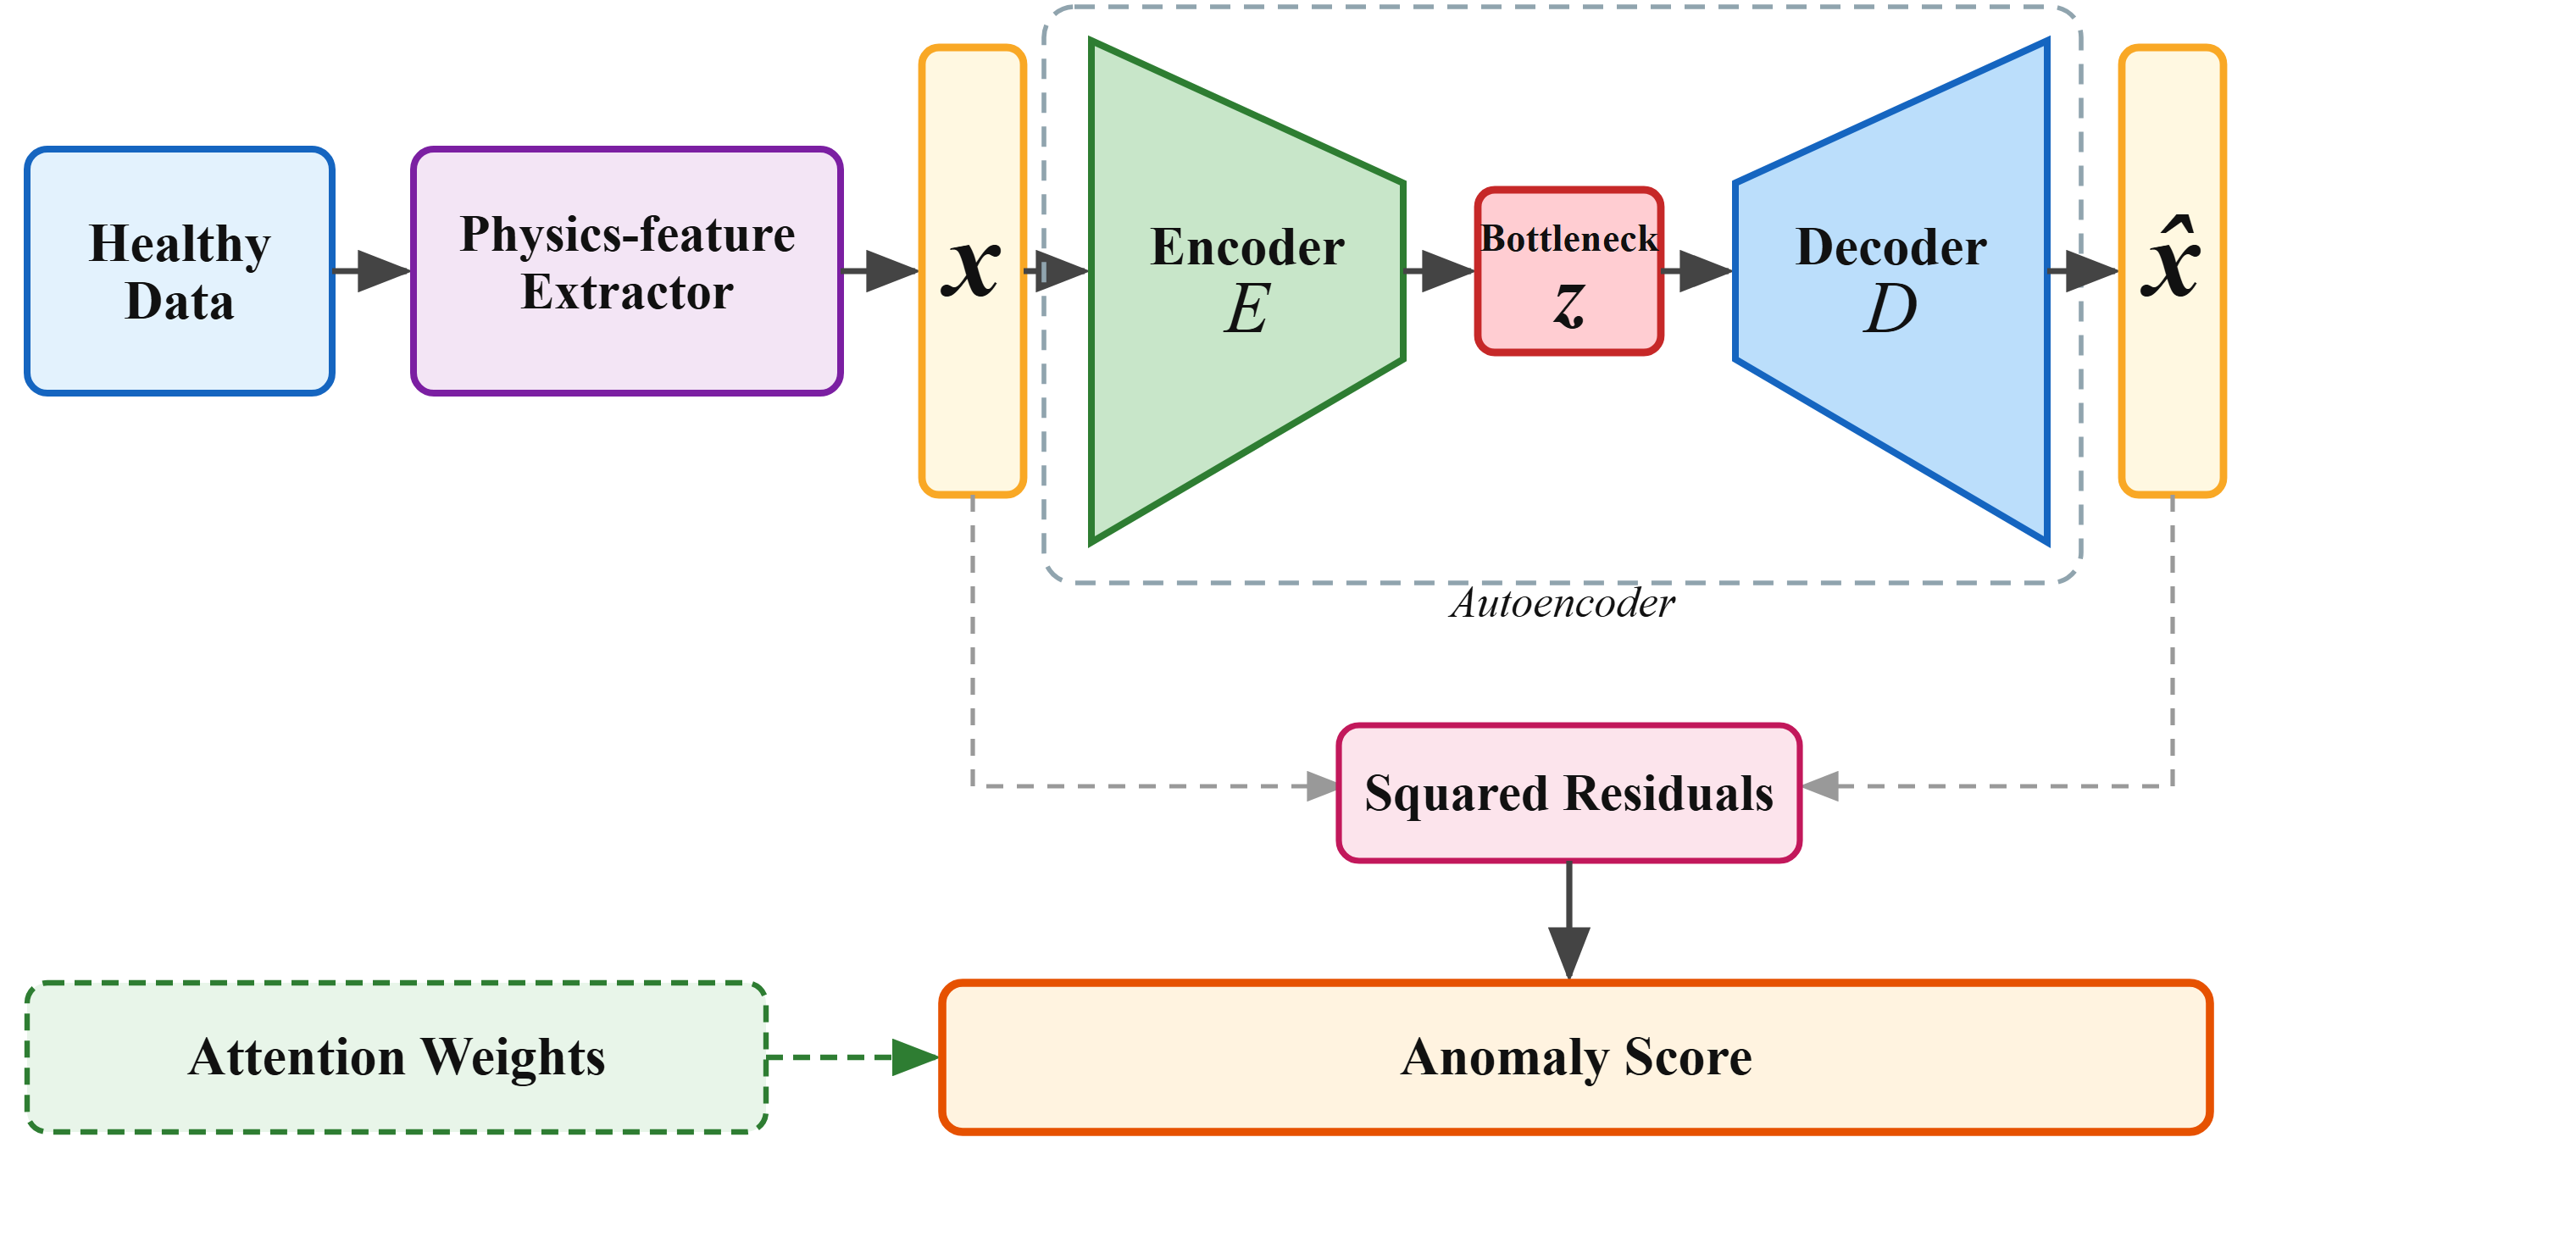
\includegraphics[width=\linewidth]{fig1.png}
\caption{End-to-end pipeline of the physics-guided autoencoder with unsupervised feature attention (PGAE-A).}
\label{fig:overview}
\end{figure}

Figure~\ref{fig:overview} summarizes the complete pipeline, from feature
extraction through the healthy-trained autoencoder to the attention-weighted
anomaly score. Each measurement window is represented by a feature vector
$x \in \mathbb{R}^{d}$ of physics-motivated vibration descriptors. The qualifier \emph{physics-guided} refers to this
input representation rather than to the network architecture: the coordinates of
$x$ are interpretable vibration descriptors drawn from three domains---time-domain
statistics, power-spectral-density (PSD) shape descriptors, and inter-sensor
transmissibility ratios---whose sensitivity to stiffness loss is mechanistically
motivated, in contrast to raw stochastic waveforms. All coordinates are
standardized to zero mean and unit variance, so that no descriptor dominates the
reconstruction objective merely by virtue of its numerical scale.

Because operational monitoring provides only healthy-state observations, we adopt
a reconstruction-based one-class formulation. An autoencoder trained to reproduce
healthy feature vectors learns a compact model of the healthy operating condition:
a window consistent with that condition is reconstructed accurately, whereas a
window carrying damage-induced deviations is not, so the reconstruction residual
supplies the raw anomaly signal. This residual is available separately for each
feature, which is precisely what allows the attention mechanism introduced below
to re-weight the descriptors coordinate by coordinate.

The backbone is a symmetric, fully connected autoencoder consisting of an encoder
$E_\phi$ and a decoder $D_\psi$ (Figure~\ref{fig:ae_arch}). The encoder compresses
the input through successive hidden layers into a low-dimensional latent code $z$,
and the decoder mirrors this structure to return a reconstruction
$\hat{x} \in \mathbb{R}^{d}$. The narrow bottleneck forces the network to encode
only the reproducible regularities of the healthy state rather than to memorize
individual windows. Writing $a^{(0)} = x$, each hidden layer applies an affine
map followed by a ReLU nonlinearity,
\begin{equation}
a^{(l)} \;=\; \mathrm{ReLU}\!\bigl(W^{(l)} a^{(l-1)} + b^{(l)}\bigr),
\qquad l = 1,\dots,L,
\label{eq:layer}
\end{equation}
so that the encoder and decoder are the compositions
\begin{equation}
z \;=\; E_\phi(x), \qquad \hat{x} \;=\; D_\psi(z) \;=\; D_\psi\!\bigl(E_\phi(x)\bigr),
\label{eq:encdec}
\end{equation}
where $\phi$ and $\psi$ collect the layer weights $\{W^{(l)}, b^{(l)}\}$ of the two
stacks; the output layer is affine, leaving the reconstruction unconstrained in
sign and range.

The model is trained exclusively on the healthy training windows $\mathcal{T}$ by
minimizing the mean squared reconstruction error
\begin{equation}
\mathcal{L}(\phi,\psi) \;=\;
\frac{1}{|\mathcal{T}|}\sum_{x \in \mathcal{T}}
\bigl\lVert x - D_\psi\!\bigl(E_\phi(x)\bigr) \bigr\rVert_2^2 ,
\label{eq:loss}
\end{equation}
by gradient-based optimization. To prevent overfitting on the limited healthy
data, training is stopped early once the loss on a separate healthy validation
split ceases to improve, and the parameters attaining the lowest validation loss
are retained. No damaged window and no label enters this stage.

The quantity on which detection ultimately rests is the per-feature reconstruction
residual
\begin{equation}
r(x) \;=\; x - \hat{x} \;=\; x - D_\psi\!\bigl(E_\phi(x)\bigr) \in \mathbb{R}^{d},
\label{eq:residual}
\end{equation}
whose $i$-th coordinate $r_i(x) = x_i - \hat{x}_i$ quantifies how far feature $i$
departs from \textcolor{red}{the value the autoencoder reconstructs for it}. All subsequent
scoring---both the plain baseline and the attention mechanism---is a function of
this residual vector alone.

\begin{figure}[htbp]
\centering
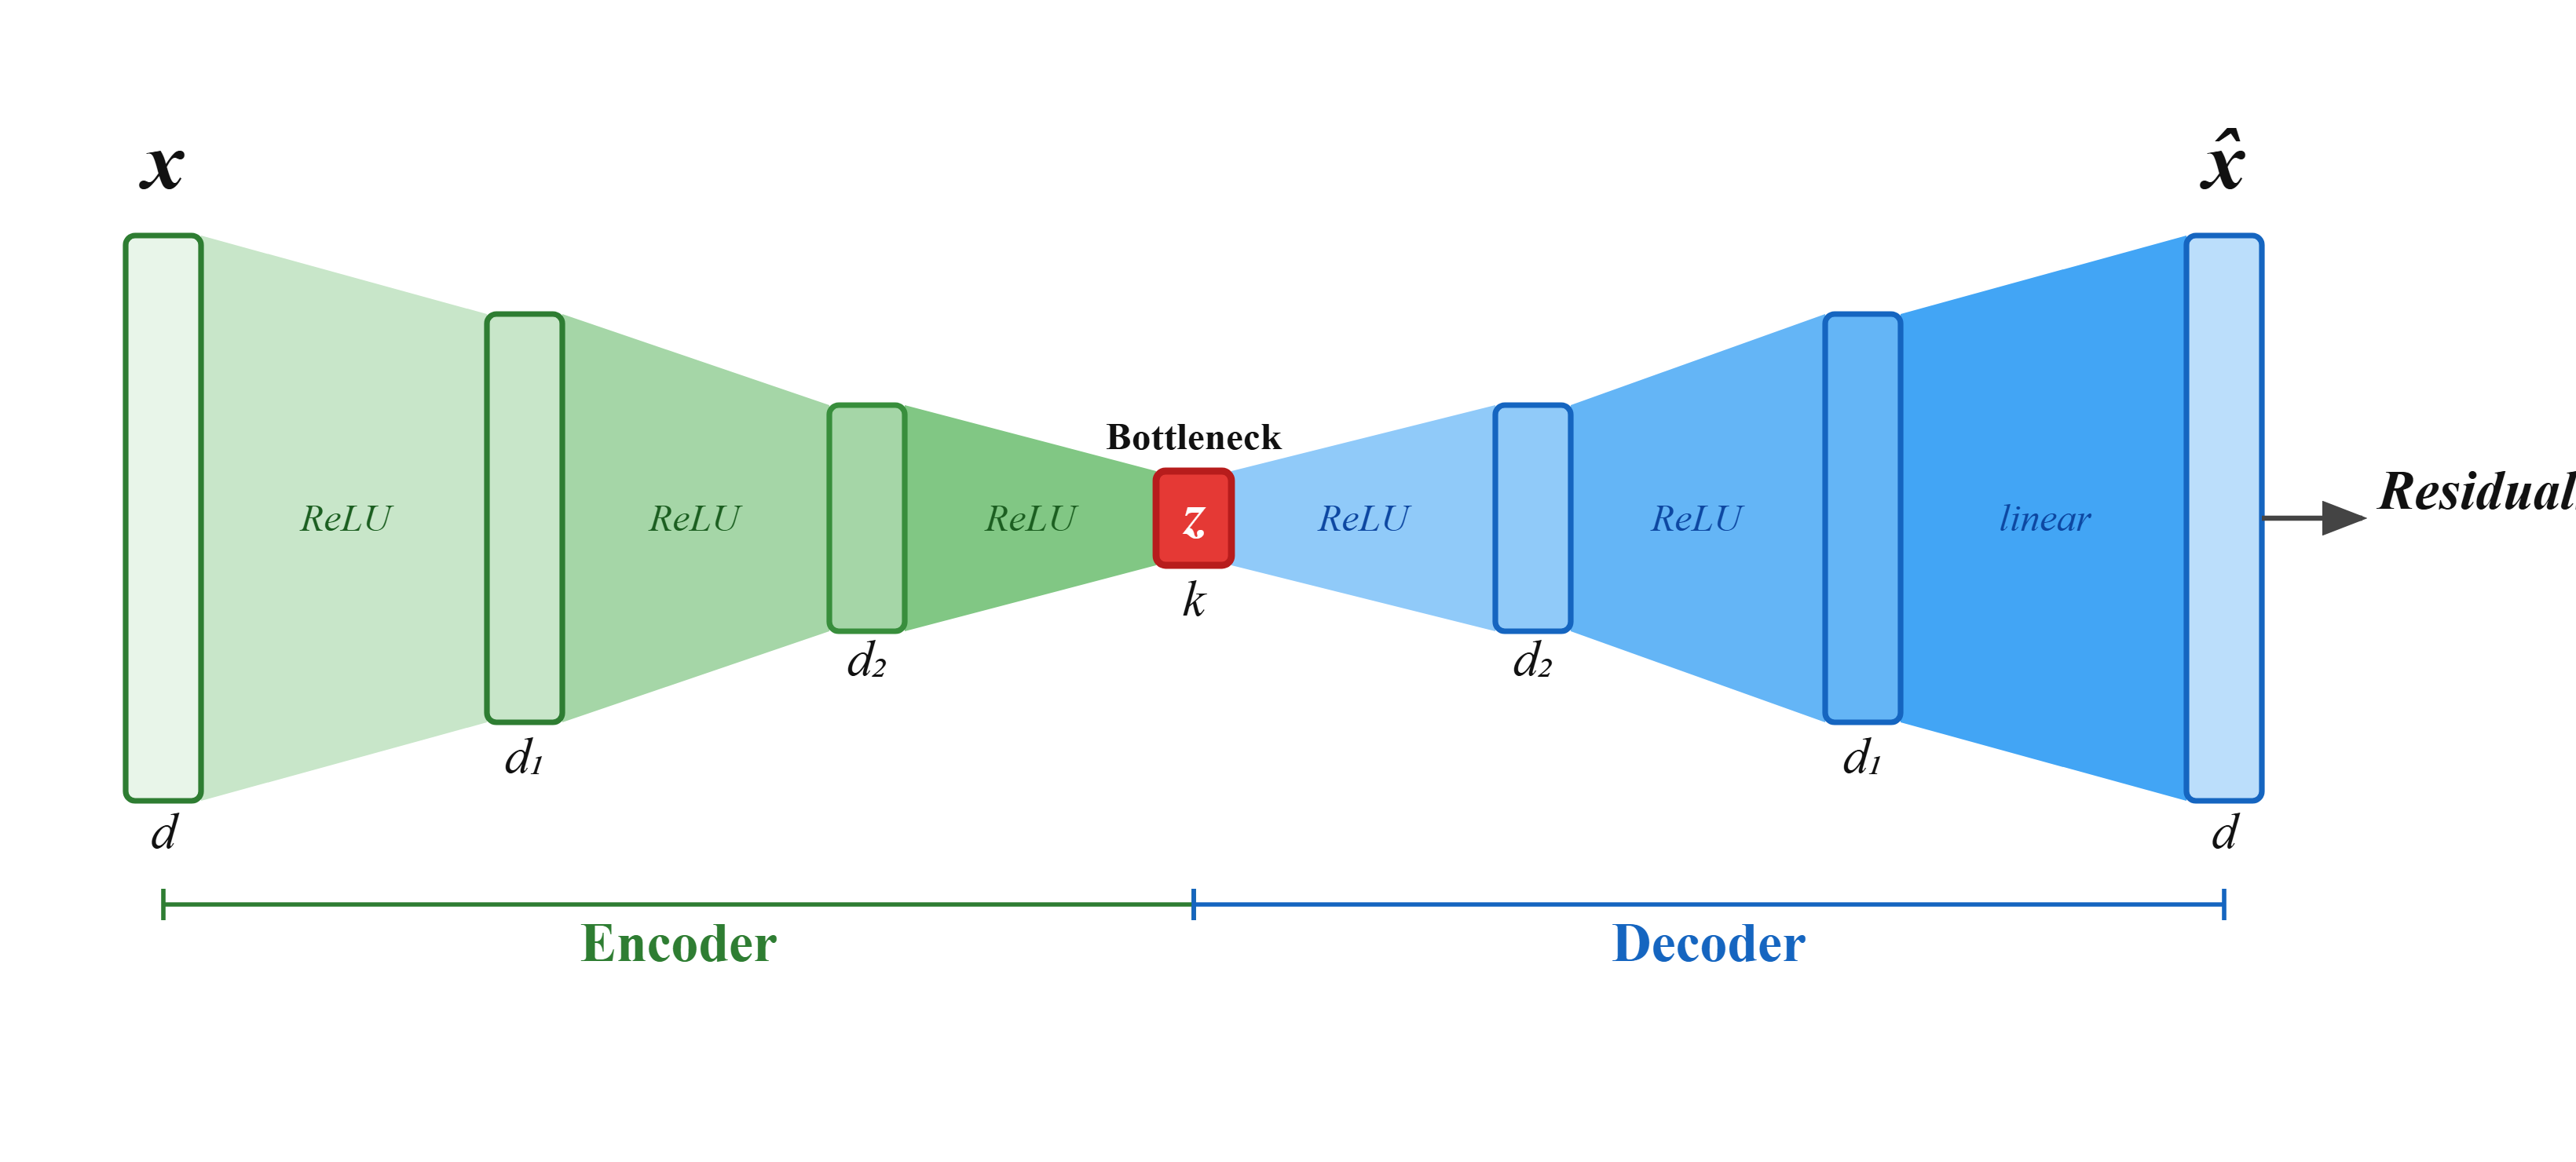
\includegraphics[width=\linewidth]{fig2.png}
\caption{Autoencoder backbone.}
\label{fig:ae_arch}
\end{figure}

\subsection{Unsupervised feature attention}
\label{sec:attention}
Weighting every feature equally does not work on a bank this large. The plain
anomaly score $s(x)=\sum_i r_i^2$ treats all coordinates alike, so it is
dominated by the features whose healthy-state residuals are largest.
\textcolor{red}{Such a large residual can arise for several reasons---environmental
and operational variability \cite{martinsanz2020,entezami2026meta}, sensor
noise, nonlinear response, or simply insufficient model capacity---and this
work does not distinguish between them; any of these is a reason the
autoencoder is not expected to reproduce that feature accurately.} Their large fluctuations
in the healthy state drown out the small deviations of features that
\textcolor{red}{are reconstructed reliably in the healthy state}---and it is those small deviations that carry the damage
signal.

A criterion is available that uses the healthy state alone: how reliably each
feature is reconstructed under normal conditions. Let
\begin{equation}
\overline{r_i^2} \;=\; \frac{1}{|\mathcal{T}|}\sum_{x\in\mathcal{T}}
\bigl(x_i - \hat{x}_i\bigr)^2
\label{eq:meanres}
\end{equation}
denote the mean squared reconstruction residual of feature $i$ over the healthy
training set $\mathcal{T}$. A small $\overline{r_i^2}$ indicates that
\textcolor{red}{feature $i$ is reconstructed reliably in the healthy state}, so that a subsequent deviation is
informative, whereas a large $\overline{r_i^2}$ indicates a feature that is poorly
predicted even in the healthy condition. The attention weights and the weighted
anomaly score are defined accordingly as
\begin{equation}
a_i \;=\;
\frac{\exp\!\bigl(-\overline{r_i^2}/\beta\bigr)}
     {\sum_{j} \exp\!\bigl(-\overline{r_j^2}/\beta\bigr)},
\qquad
s(x) \;=\; \sum_{i} a_i\,\bigl(x_i-\hat{x}_i\bigr)^2 ,
\label{eq:attention}
\end{equation}
where the sharpness parameter $\beta > 0$ (the softmax temperature) controls how
strongly the weighting concentrates: a small $\beta$ places almost all weight on
the most reliably reconstructed features, while a large $\beta$ recovers uniform
weighting and hence the plain score. Every
quantity in Eqs.~\eqref{eq:meanres}--\eqref{eq:attention} is computed from healthy
data alone, so that no damaged window and no label enters the construction.

The sharpness parameter $\beta$ must likewise be selected without damage labels, or the
one-class property is lost. It is fixed from the shape of the
\emph{participation ratio} $\mathrm{PR}(\beta) = 1/\sum_i a_i^2$, which measures
the effective number of features retained by the attention and depends only on
the healthy residuals $\{\overline{r_i^2}\}$. As a function of $\log\beta$,
$\mathrm{PR}(\beta)$ is a monotone sigmoid: it rises from a
small baseline, where attention concentrates sharply on a few features,
through a region of fastest growth, to a plateau at $\mathrm{PR}\!\approx\!d$,
where weighting is uniform. Two landmarks are
intrinsic to this curve and require nothing to be chosen by hand: the \emph{lower knee},
where $\mathrm{PR}$ departs from its baseline, obtained by the standard
knee-detection (Kneedle) construction on the normalized curve; and the
\emph{inflection}, where $\mathrm{PR}$ grows fastest, i.e.\ the maximum of
$\mathrm{d}\,\mathrm{PR}/\mathrm{d}\!\log\beta$. Below the lower knee the
attention collapses onto degenerate coordinates; above the inflection it
\textcolor{red}{admits the unreliable, high-residual features that plain
scoring cannot handle.} The two landmarks therefore bracket the useful operating range, and we
set $\beta$ at the midpoint of this window on the $\log\beta$ axis---the
geometric mean of the two endpoints, which is the scale-invariant centre for a
parameter of this kind. The procedure is fully automatic and one-class: it
introduces no target retention fraction and never inspects a damaged window.
\textcolor{red}{We report the retention as a fraction of the bank,
$\alpha = \mathrm{PR}(\beta^{*})/d$; like $\beta^{*}$ itself, $\alpha$ is an
output of this rule, not a value chosen in advance.}
Section~\ref{sec:mechanism} carries out this selection on the Z24 healthy
residuals and reports the resulting $\beta$.

% =====================================================================
\section{Experiments and Results}
\label{sec:data}

Let $\mathcal{X}_H$ denote the set of measurements acquired from the healthy
structure. Each detector is trained on a subset of $\mathcal{X}_H$ only and, at
test time, assigns to every window an anomaly score that is expected to be
higher for damaged windows than for healthy ones. Under the one-class protocol
adopted here, no damaged example and no health-state label is used at any stage
of training, feature selection, or model selection. Baselines that relax this
constraint are identified explicitly, and the performance advantage they obtain
from access to labels is quantified.

\subsection{The Z24 bridge benchmark}
The Z24 was a post-tensioned concrete box-girder bridge in the canton of Bern,
Switzerland, forming part of the road link between the villages of Koppigen and
Utzenstorf. It comprised a $30$~m main span and two $14$~m side spans. Prior to
its demolition at the end of 1998, the bridge was used as a full-scale
damage-detection benchmark under a European research programme, in which
seventeen progressively more severe damage scenarios were deliberately
introduced over August--September 1998 and ambient-vibration tests were
performed after each state \cite{reynders2015}. The controlled, well-documented
progression from an intact structure to severe prestressing-system failure, on a
real full-scale bridge, is what makes Z24 the field's most widely used
damage-detection benchmark.

The structure was instrumented with accelerometers recorded over several sensor
setups; five channels remained in fixed positions across all setups and are the
only channels used here, sampled at $100$~Hz. They are denoted R1V, R2L, R2T,
R2V and R3V, where R1--R3 are reference points along the deck and V, L and T
indicate the vertical, longitudinal and transverse measurement directions.
Following benchmark convention \cite{abdrabo2024}, the first eight states---the
undamaged references, the progressive pier settlements of up to $95$~mm, and the
re-referencing after the pier was restored---are treated as \emph{healthy},
since they induce only minor and largely reversible changes in the dynamic
response. States 9--17---concrete spalling, an abutment landslide, failure of
concrete hinges and of anchor heads, and the progressive rupture of prestressing
tendons---are treated as \emph{damaged}, as they progressively compromise the
load-carrying system. Figure~\ref{fig:z24} shows the sensor layout, and
Table~\ref{tab:states} lists the seventeen states with their health/damage
assignment; the dataset is publicly available from KU Leuven.

\begin{figure}[htbp]
\centering
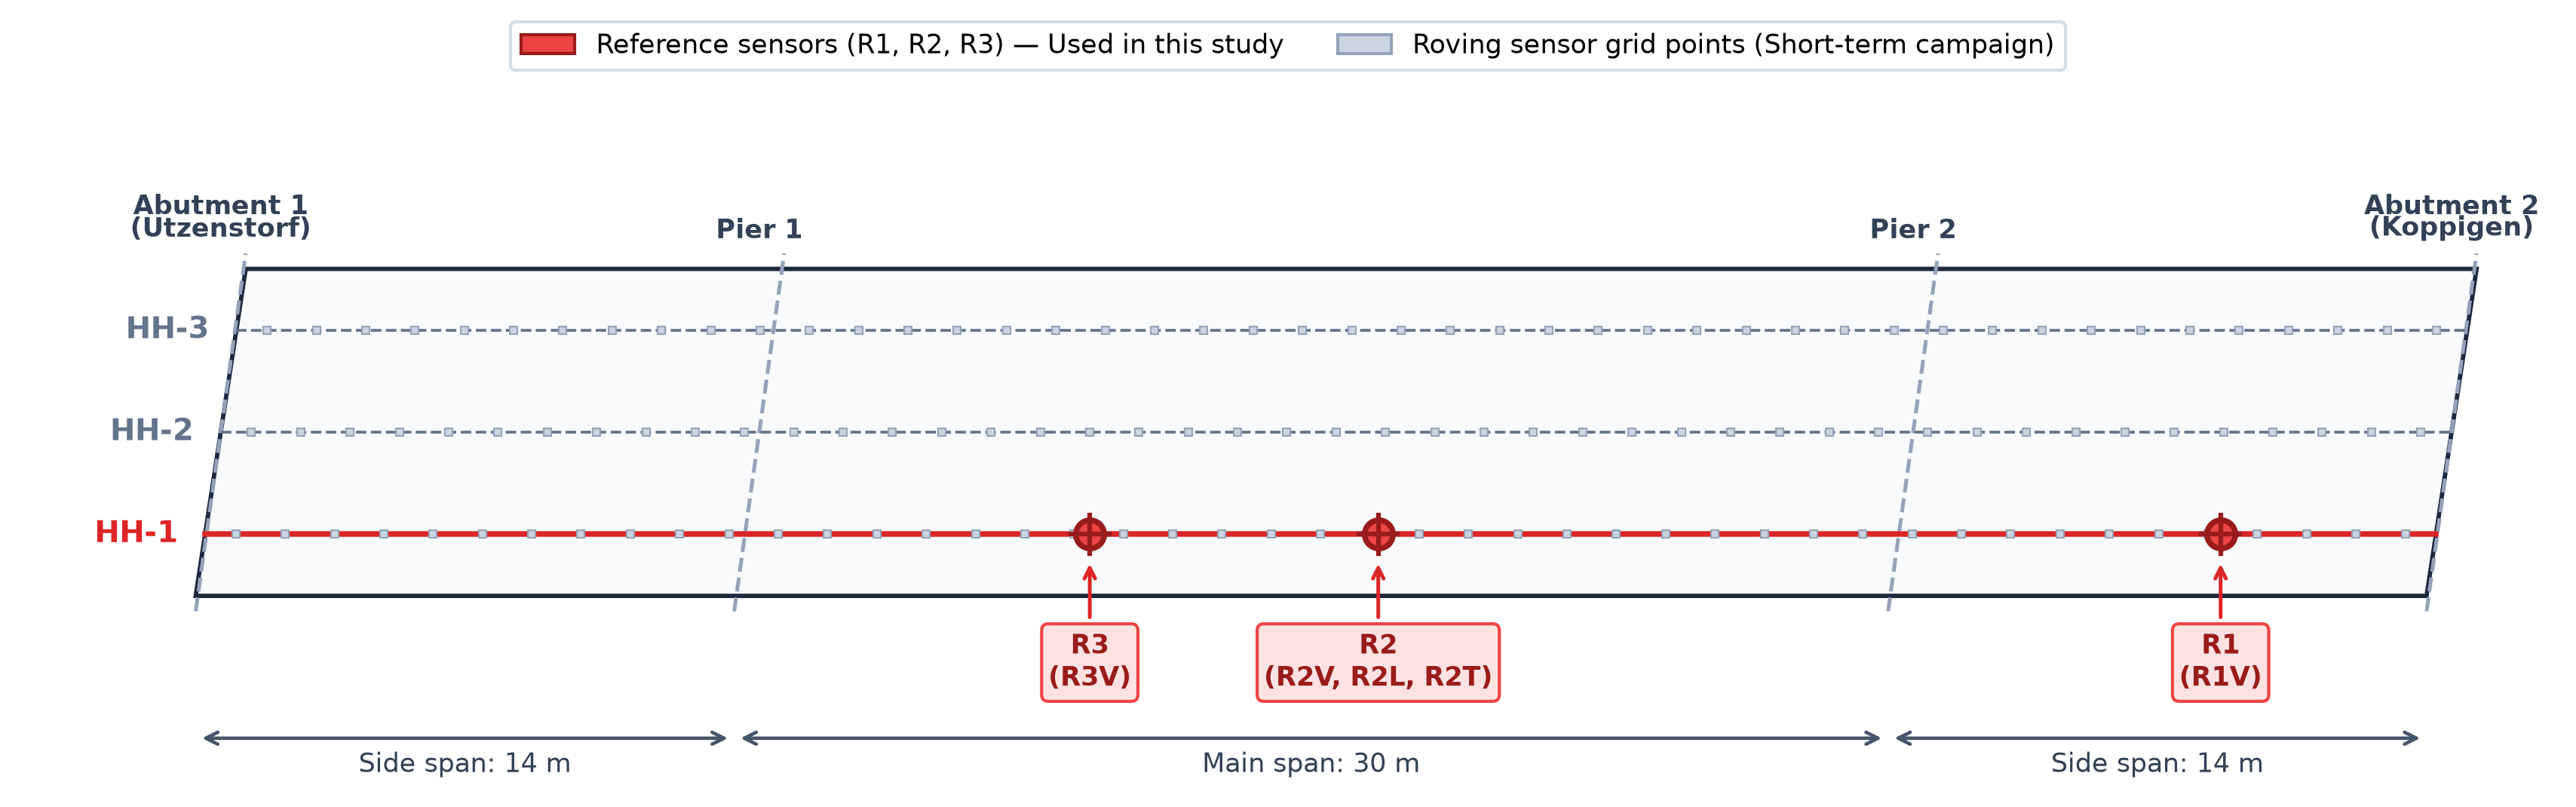
\includegraphics[width=\linewidth]{fig3.png}
\caption{Sensor grid of the Z24 short-term monitoring campaign. Only the three
reference sensors R1, R2 and R3 (marked in red at the positions shown) are used
in this study, as they are the only sensors that kept a fixed location across
all measurement setups.}
\label{fig:z24}
\end{figure}

\begin{table}[htbp]
\centering
\caption{The seventeen Z24 bridge states (S1--S8 healthy; S9--S17 progressive damage).}
\label{tab:states}
\small
\begin{tabular}{@{}clc@{}}
\toprule
State & Condition / scenario & Class \\
\midrule
1  & Undamaged reference                     & Healthy \\
2  & Reference (settlement system installed) & Healthy \\
3  & Reference measurement                   & Healthy \\
4  & Pier settlement, 20~mm                  & Healthy \\
5  & Pier settlement, 40~mm                  & Healthy \\
6  & Pier settlement, 80~mm                  & Healthy \\
7  & Pier settlement, 95~mm                  & Healthy \\
8  & Pier lifted; new reference              & Healthy \\
\midrule
9  & Concrete spalling, 12~m$^2$             & Damaged \\
10 & Concrete spalling, 24~m$^2$             & Damaged \\
11 & Landslide at abutment                   & Damaged \\
12 & Failure of a concrete hinge             & Damaged \\
13 & Failure of 2 anchor heads               & Damaged \\
14 & Failure of 4 anchor heads               & Damaged \\
15 & Rupture of 54 tendon wires              & Damaged \\
16 & Rupture of 100 tendon wires             & Damaged \\
17 & Rupture of 154 tendon wires             & Damaged \\
\bottomrule
\end{tabular}
\end{table}

\subsection{Physics-feature bank}
\label{sec:features}
The five channels of each state are concatenated across setups
\textcolor{red}{and, for the states whose setups fall short of the
$589{,}824$-sample target length, extended to it by repeating their initial
samples} and segmented into $36$ non-overlapping windows of
$16{,}384$ samples ($\approx163.8$~s). This gives $612$ windows in total,
$36$ per state, of which $288$ are healthy (states 1--8) and $324$ are damaged
(states 9--17). We adopt the benchmark's fixed per-state partition into a
$544$-window training pool and a $68$-window test pool. Because this partition
predates the one-class setting, each pool mixes classes: the training pool holds
$256$ healthy and $288$ damaged windows, the test pool $32$ healthy and $36$
damaged. The one-class detectors never use damaged windows for training---the
autoencoder is fit only on the $256$ healthy training-pool windows---while all
$324$ damaged windows together with the $32$ healthy test windows serve
exclusively for evaluation.

From each window we extract a large and deliberately redundant bank of
physics-motivated descriptors. The descriptors fall into three groups---one in
the time domain and two in the frequency domain---whose counts are collected in
Table~\ref{tab:features}.

The time-domain group summarizes each detrended channel by $49$ scalar
statistics: statistical moments (mean, median, variance, skewness, kurtosis, mode),
length- and repetition-based counts (zero crossings, longest run above the
mean, short-lag peak counts), autocorrelation and signal-complexity metrics,
statistical combinations (root-mean-square, mean absolute change between
adjacent samples, central second-difference estimates), and moving-average
features. Applied to all five channels, this group contributes $49\times5=245$
features.

The first frequency-domain group describes the power spectral density (PSD) of
each channel, estimated by Welch's method as $S_x(f)=|X(f)|^2$ with $X(f)$ the
discrete Fourier transform of the acceleration $x[n]$. Its shape is captured by
$74$ descriptors: descriptive statistics of the spectrum, piecewise cubic
regression coefficients, the indices, positions and heights of the largest and
sharpest peaks, peak heights within successive $2.5$~Hz sub-bands, and the
spectral centroid. These descriptors track shifts of the modal
frequencies---the classical spectral signature of stiffness loss---and
contribute $74\times5=370$ features.

The second frequency-domain group applies the same $74$ spectral descriptors to
inter-channel transmissibility functions
\begin{equation}
T_{ij}(f) \;=\; \frac{|\mathrm{PSD}_i(f)|}{|\mathrm{PSD}_j(f)|},
\label{eq:transmissibility}
\end{equation}
formed with R1V as the common reference channel $j$ \cite{johnson2002}.
\textcolor{red}{Because R1V and every other channel are driven by the same,
unmeasured ambient excitation, each response's power spectral density
factors approximately as $\mathrm{PSD}_i(f) \approx |H_i(f)|^2 S_x(f)$, where
$H_i(f)$ is the structure's own frequency response between the (unknown)
excitation and channel $i$, and $S_x(f)$ is the excitation spectrum, common
to every channel. The ratio $T_{ij}(f)$ therefore approximately cancels
$S_x(f)$ and depends only on the structure's transfer characteristics
between the two sensor locations---exactly what a local, damage-induced
change in stiffness or mass would alter, and exactly what an ambient
test, with no controlled or measured input, requires.} Transmissibility
therefore isolates relative, spatially resolved changes between sensor
locations and acts as a differential damage indicator. With four channels
(R2L, R2T, R2V, R3V) referred to R1V, this group contributes $74\times4=296$
features. \textcolor{red}{Supplementary Material S6 lists the definition and
implementation setting of every one of the $49$ time-domain and $74$
PSD/transmissibility descriptors.}

After standardization and the removal of feature columns that are not
sufficiently complete across windows, the bank comprises $d = 906$ descriptors
per window, giving benchmark feature matrices of shape $(544, 906)$ for the
training pool and $(68, 906)$ for the test pool (of which only the $256$ healthy
training-pool rows enter autoencoder training). \textcolor{red}{We fit the completeness filter (dropping any of the $906$
columns with $\geq10\%$ missing values), the missing-value imputer (column
mean, via \texttt{SimpleImputer}), and the standardization mean and variance
using only the $256$ healthy training rows; these fitted parameters are then
applied unchanged, without refitting, to the remaining $288$ damaged
training-pool windows and to the full $68$-window test pool.} As an implementation note, we accelerated the reference feature
extractor of \cite{abdrabo2024} by $2.27\times$ end to end by replacing direct
convolution with FFT-based convolution in its moving-average computations, with
bit-identical output---relevant both for reproducibility and for edge
deployment.

\begin{table}[htbp]
\centering
\caption{The 906-dimensional physics-feature bank.}
\label{tab:features}
\small
\begin{tabular}{@{}llccr@{}}
\toprule
Feature group & Domain & Per channel & Channels/pairs & Count \\
\midrule
Statistical descriptors      & Time      & 49 & 5 & 245 \\
PSD shape descriptors        & Frequency & 74 & 5 & 370 \\
Transmissibility descriptors & Frequency & 74 & 4 & 296 \\
\midrule
\multicolumn{4}{@{}l}{Raw descriptors extracted} & 911 \\
\multicolumn{4}{@{}l}{Retained (columns $\geq 90\%$ complete)} & 906 \\
\bottomrule
\end{tabular}
\end{table}

\subsection{Model training and evaluation protocol}
\label{sec:train}
All detectors are trained on the healthy training windows, split $80/20$ into a
training and a validation-normal subset. For a yes/no alarm, the threshold is
set at the 95th percentile of the validation-normal scores, so that $5\%$ of
healthy windows are flagged. It is computed from healthy data alone and applied
identically to every detector. Because no damaged window is ever used in
training, all $324$ of them are available for evaluation, together with the
$32$ healthy test windows. Since thresholding conventions differ across
detectors and this set is imbalanced, our primary metric is the threshold-free
ROC-AUC: the probability that a randomly chosen damaged window scores higher
than a randomly chosen healthy one, with $\mathrm{AUC}=0.5$ corresponding to
chance.

The autoencoder (Figure~\ref{fig:ae_arch}) uses an encoder of layer widths
$906\!\rightarrow\!512\!\rightarrow\!128\!\rightarrow\!32$ and a mirror-image
decoder, and is trained by minimizing the reconstruction loss of
Eq.~\eqref{eq:loss} with the Adam optimizer at a learning rate of $10^{-3}$.
Training runs for at most $600$ epochs and is halted once the validation loss
has not improved for $60$ consecutive epochs, retaining the weights that attain
the lowest validation loss. Figure~\ref{fig:loss} shows the learning curves:
the training loss decreases monotonically from about
$1.0$ toward $0.1$, whereas the validation loss reaches a minimum of roughly
$0.5$ near epoch~$90$ and then rises slightly. Early stopping selects the model
at this validation minimum, before the widening gap between the curves affects
the retained weights. Some gap is expected in this small-sample regime---about
two hundred healthy training windows in $906$ dimensions---because the network
can fit those particular windows far more closely than the intrinsic variability
of the healthy state allows for windows it has not seen.

\begin{figure}[htbp]
\centering
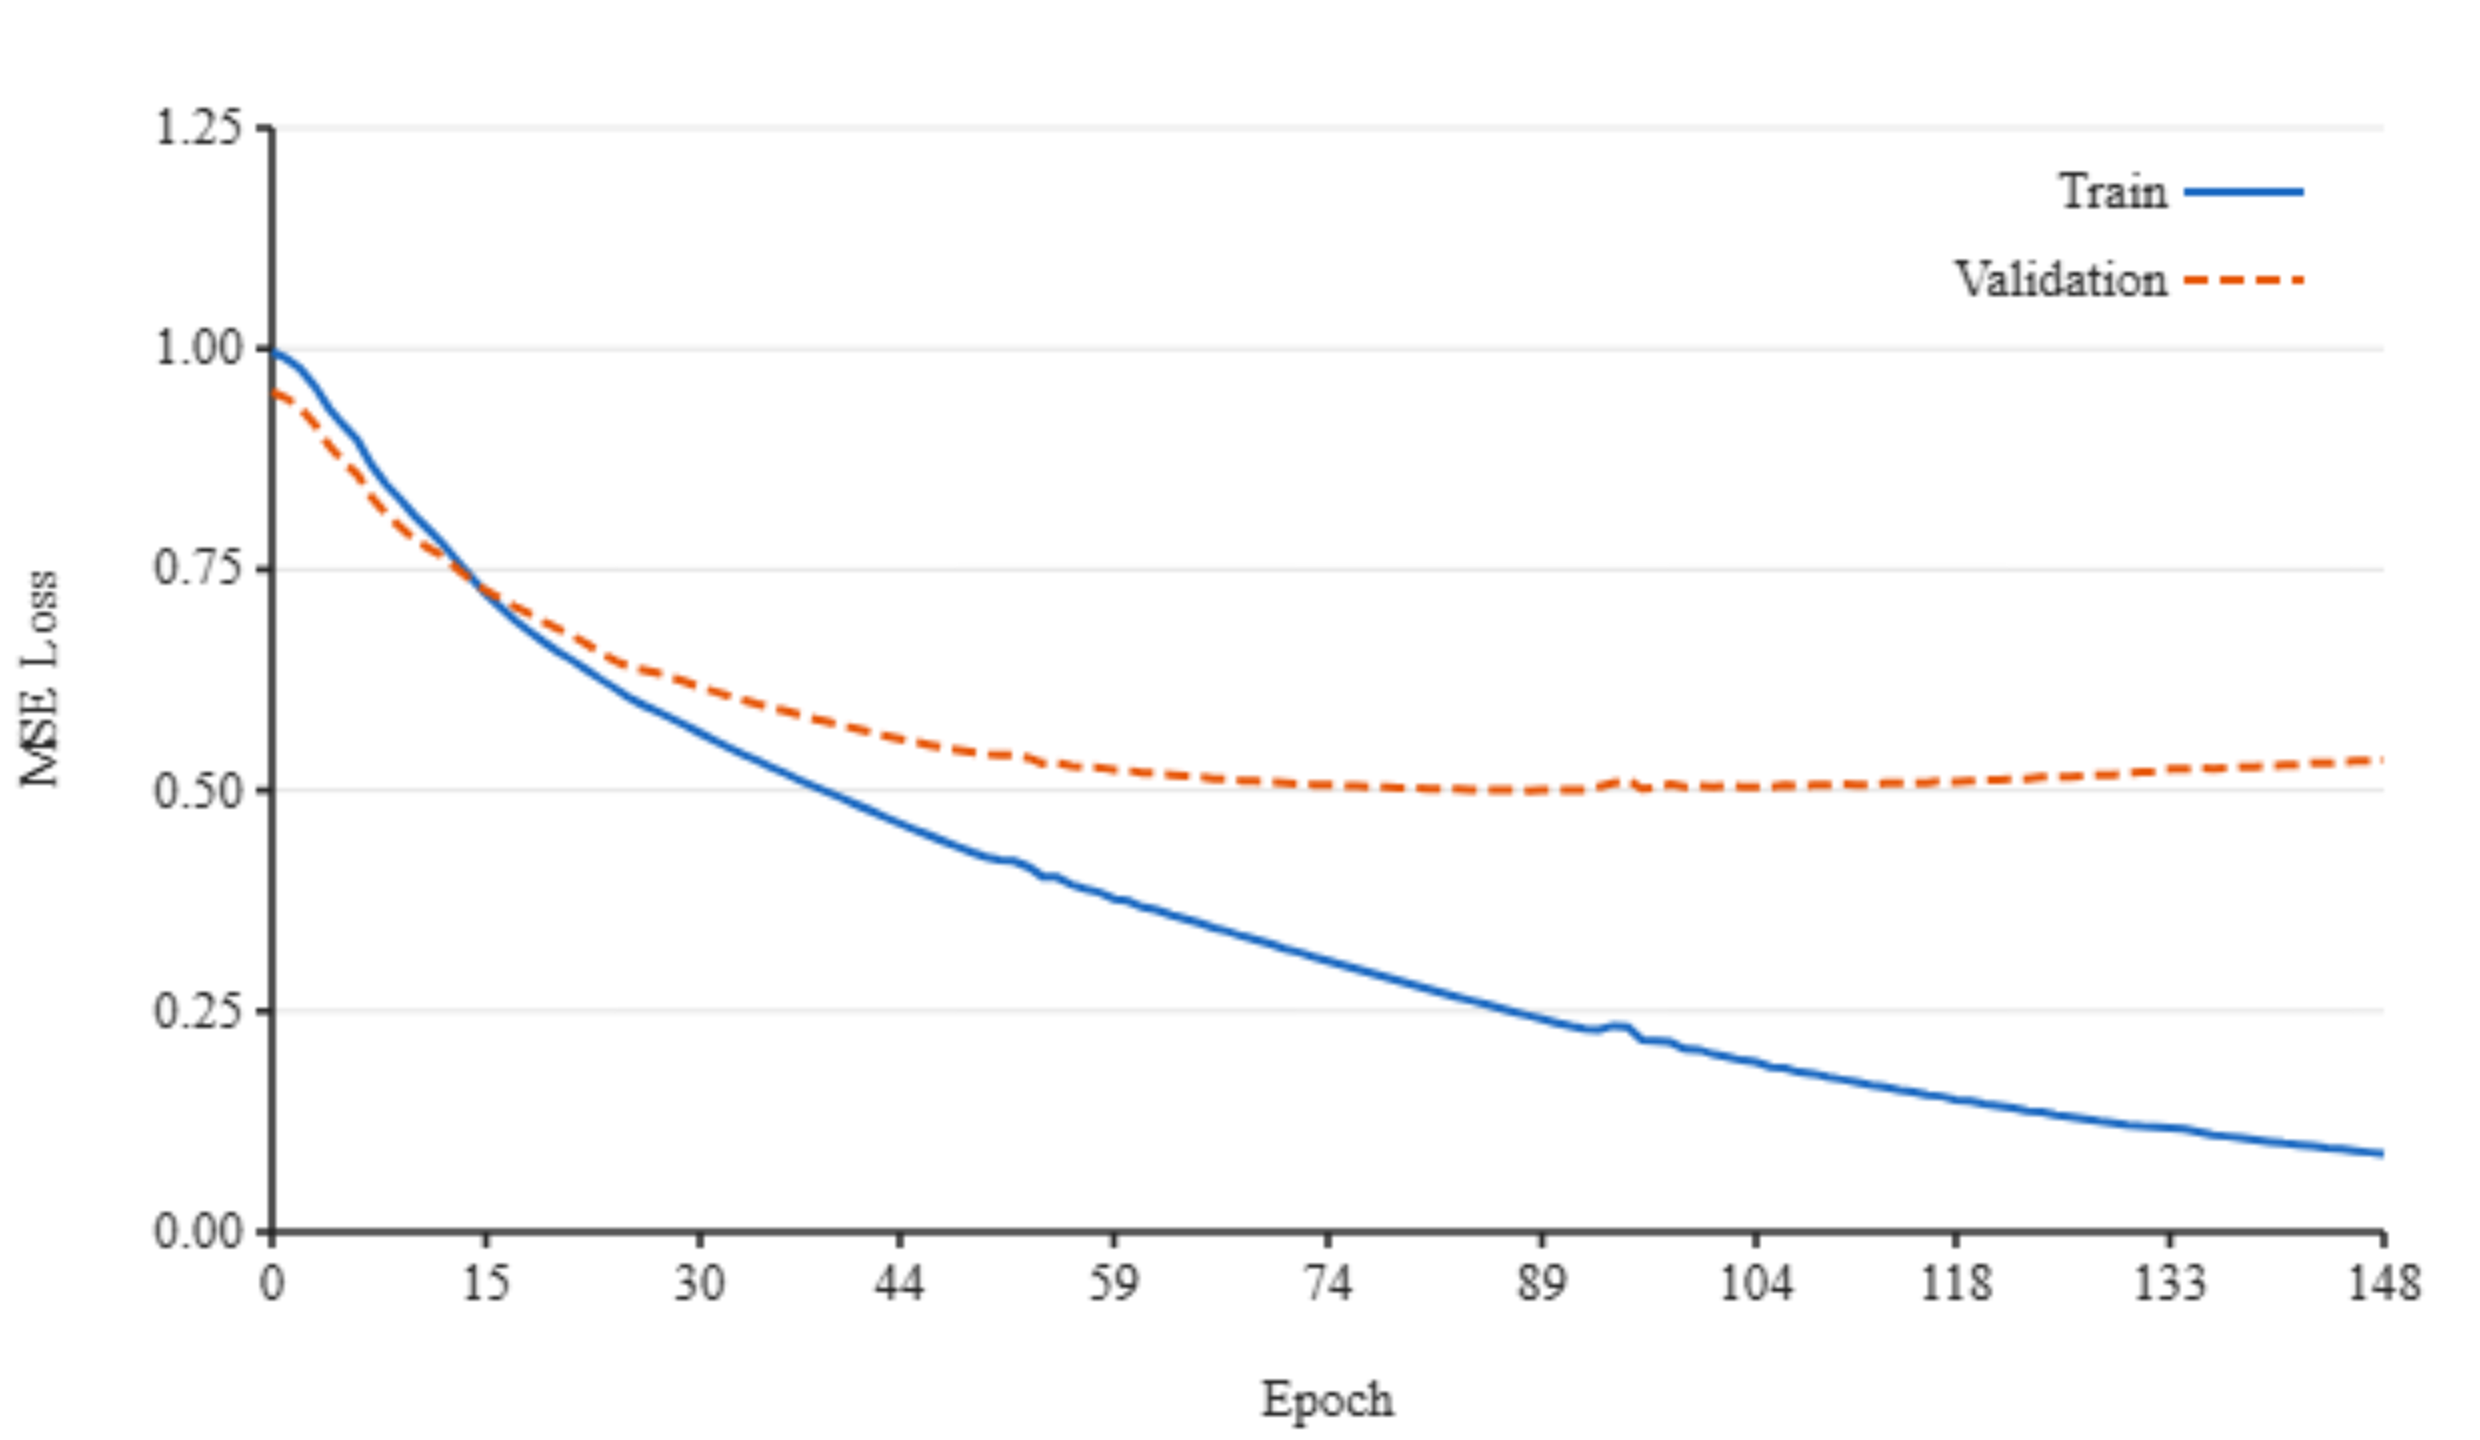
\includegraphics[width=0.72\linewidth]{fig4.png}
\caption{Training and validation reconstruction loss over epochs.}
\label{fig:loss}
\end{figure}

\subsection{One-class attention mechanism}
\label{sec:mechanism}
All figures and tables in this subsection come from a single representative run.
The attention sharpness parameter is selected automatically from the
participation-ratio curve.
Figure~\ref{fig:beta}(top) shows $\mathrm{PR}(\beta)$
computed from the Z24 healthy training residuals. Its lower knee falls at
$\beta\approx0.023$ and its inflection at $\beta\approx0.155$; these bracket the
operating window, and $\beta$ is placed at its geometric mean,
$\beta^{*}\approx0.060$, at which $\mathrm{PR}(\beta^{*})\approx277$.
The lower panel overlays the AUC as a function of
$\beta$---which requires labels and is shown for validation only---and confirms
that the automatically selected $\beta^{*}$ coincides with the performance
optimum, giving $\mathrm{AUC}=0.802$ for this run.
\textcolor{red}{These residuals come from the same healthy windows used to
train the autoencoder; Supplementary Material S2 recomputes $\beta$ and the
attention weights from an independent, held-out healthy subset and finds
detection performance unchanged.}

\begin{figure}[htbp]
\centering
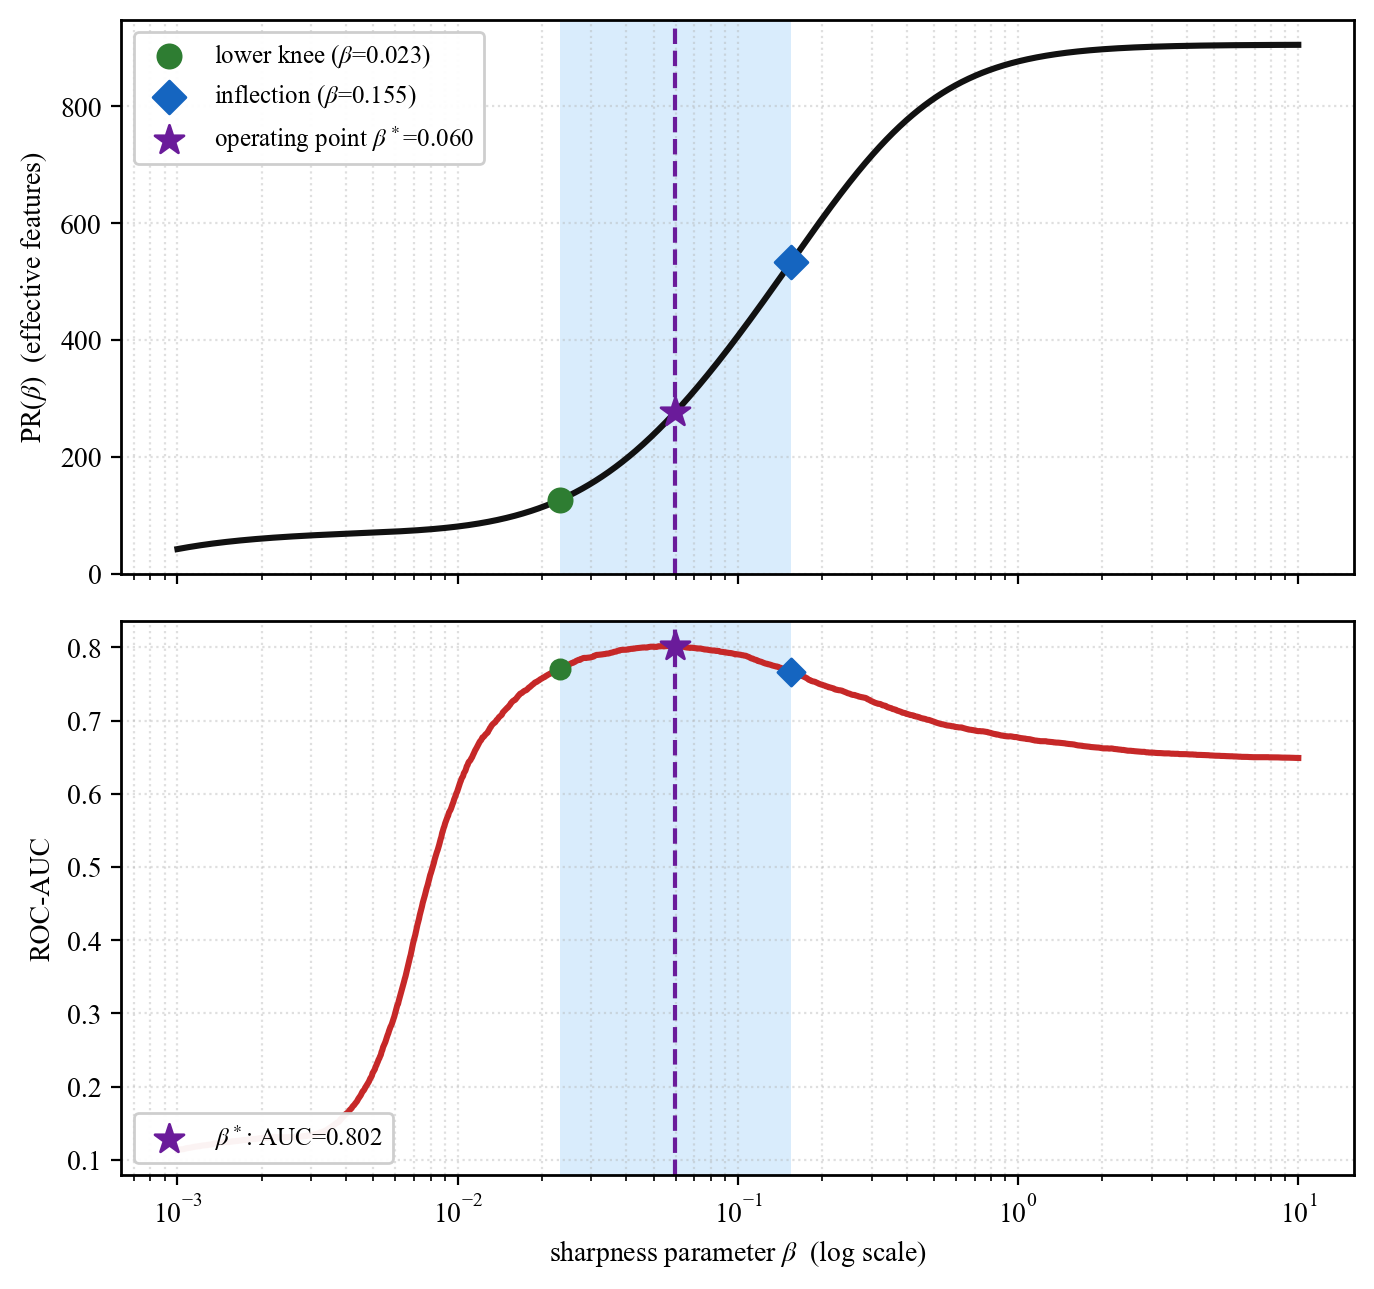
\includegraphics[width=0.82\linewidth]{fig5.png}
\caption{Automatic, one-class selection of the attention sharpness parameter $\beta$.
(top)~$\mathrm{PR}(\beta)$ from healthy residuals; the lower knee and inflection
(shaded window) bracket the useful range, and $\beta^{*}$ is set at the window's
log-scale midpoint. (bottom)~\textcolor{red}{a post-hoc diagnostic,} ROC-AUC vs.\ $\beta$ \textcolor{red}{computed on the evaluation set using damage labels for validation only and not used by the selection rule itself,}
confirms that $\beta^{*}$ lands at the optimum.}
\label{fig:beta}
\end{figure}

We now identify which features actually carry the detection signal. The
attention weight $a_i$ on its own is a poor measure of a feature's importance. A
few features in the bank are constant across every window---an artifact of how
the bank was built. Because they are reconstructed with zero error, they receive
the largest attention weights; but a feature that never varies cannot separate
healthy from damaged windows, so it adds nothing to detection.
\textcolor{red}{Supplementary Material S1 tests this directly by removing the
constant features and retraining; detection AUC is unaffected.}

A better measure is how much each feature adds to the gap between the mean
damaged score and the mean healthy score. We split that gap across features as
$\Delta_i = \mathbb{E}_{\text{damaged}}[a_i r_i^2] -
\mathbb{E}_{\text{healthy}}[a_i r_i^2]$, so that the $\Delta_i$ sum exactly to the
total gap. Figure~\ref{fig:attn} shows these contributions; of the twenty largest
(Table~\ref{tab:top20}), eighteen are PSD and transmissibility descriptors and
only two are time-domain---mirroring the finding in Table~\ref{tab:blocks} that
those two blocks outperform time-domain statistics.
\textcolor{red}{One of the two time-domain contributors, the coefficient of
variation (rank $4$, Table~\ref{tab:top20}), is computed by the standard
\texttt{tsfresh} \texttt{variation\_coefficient} function (Supplementary
Material S6) rather than custom code. Across all $612$ windows this column
has no NaN or infinite value, but one window has a standardized value
$22.9$ times the column's standard deviation, consistent with the
near-zero detrended mean that can make this ratio numerically unstable; the
remaining $611$ windows fall within $\pm 3$ standard deviations.}

\begin{figure}[htbp]
\centering
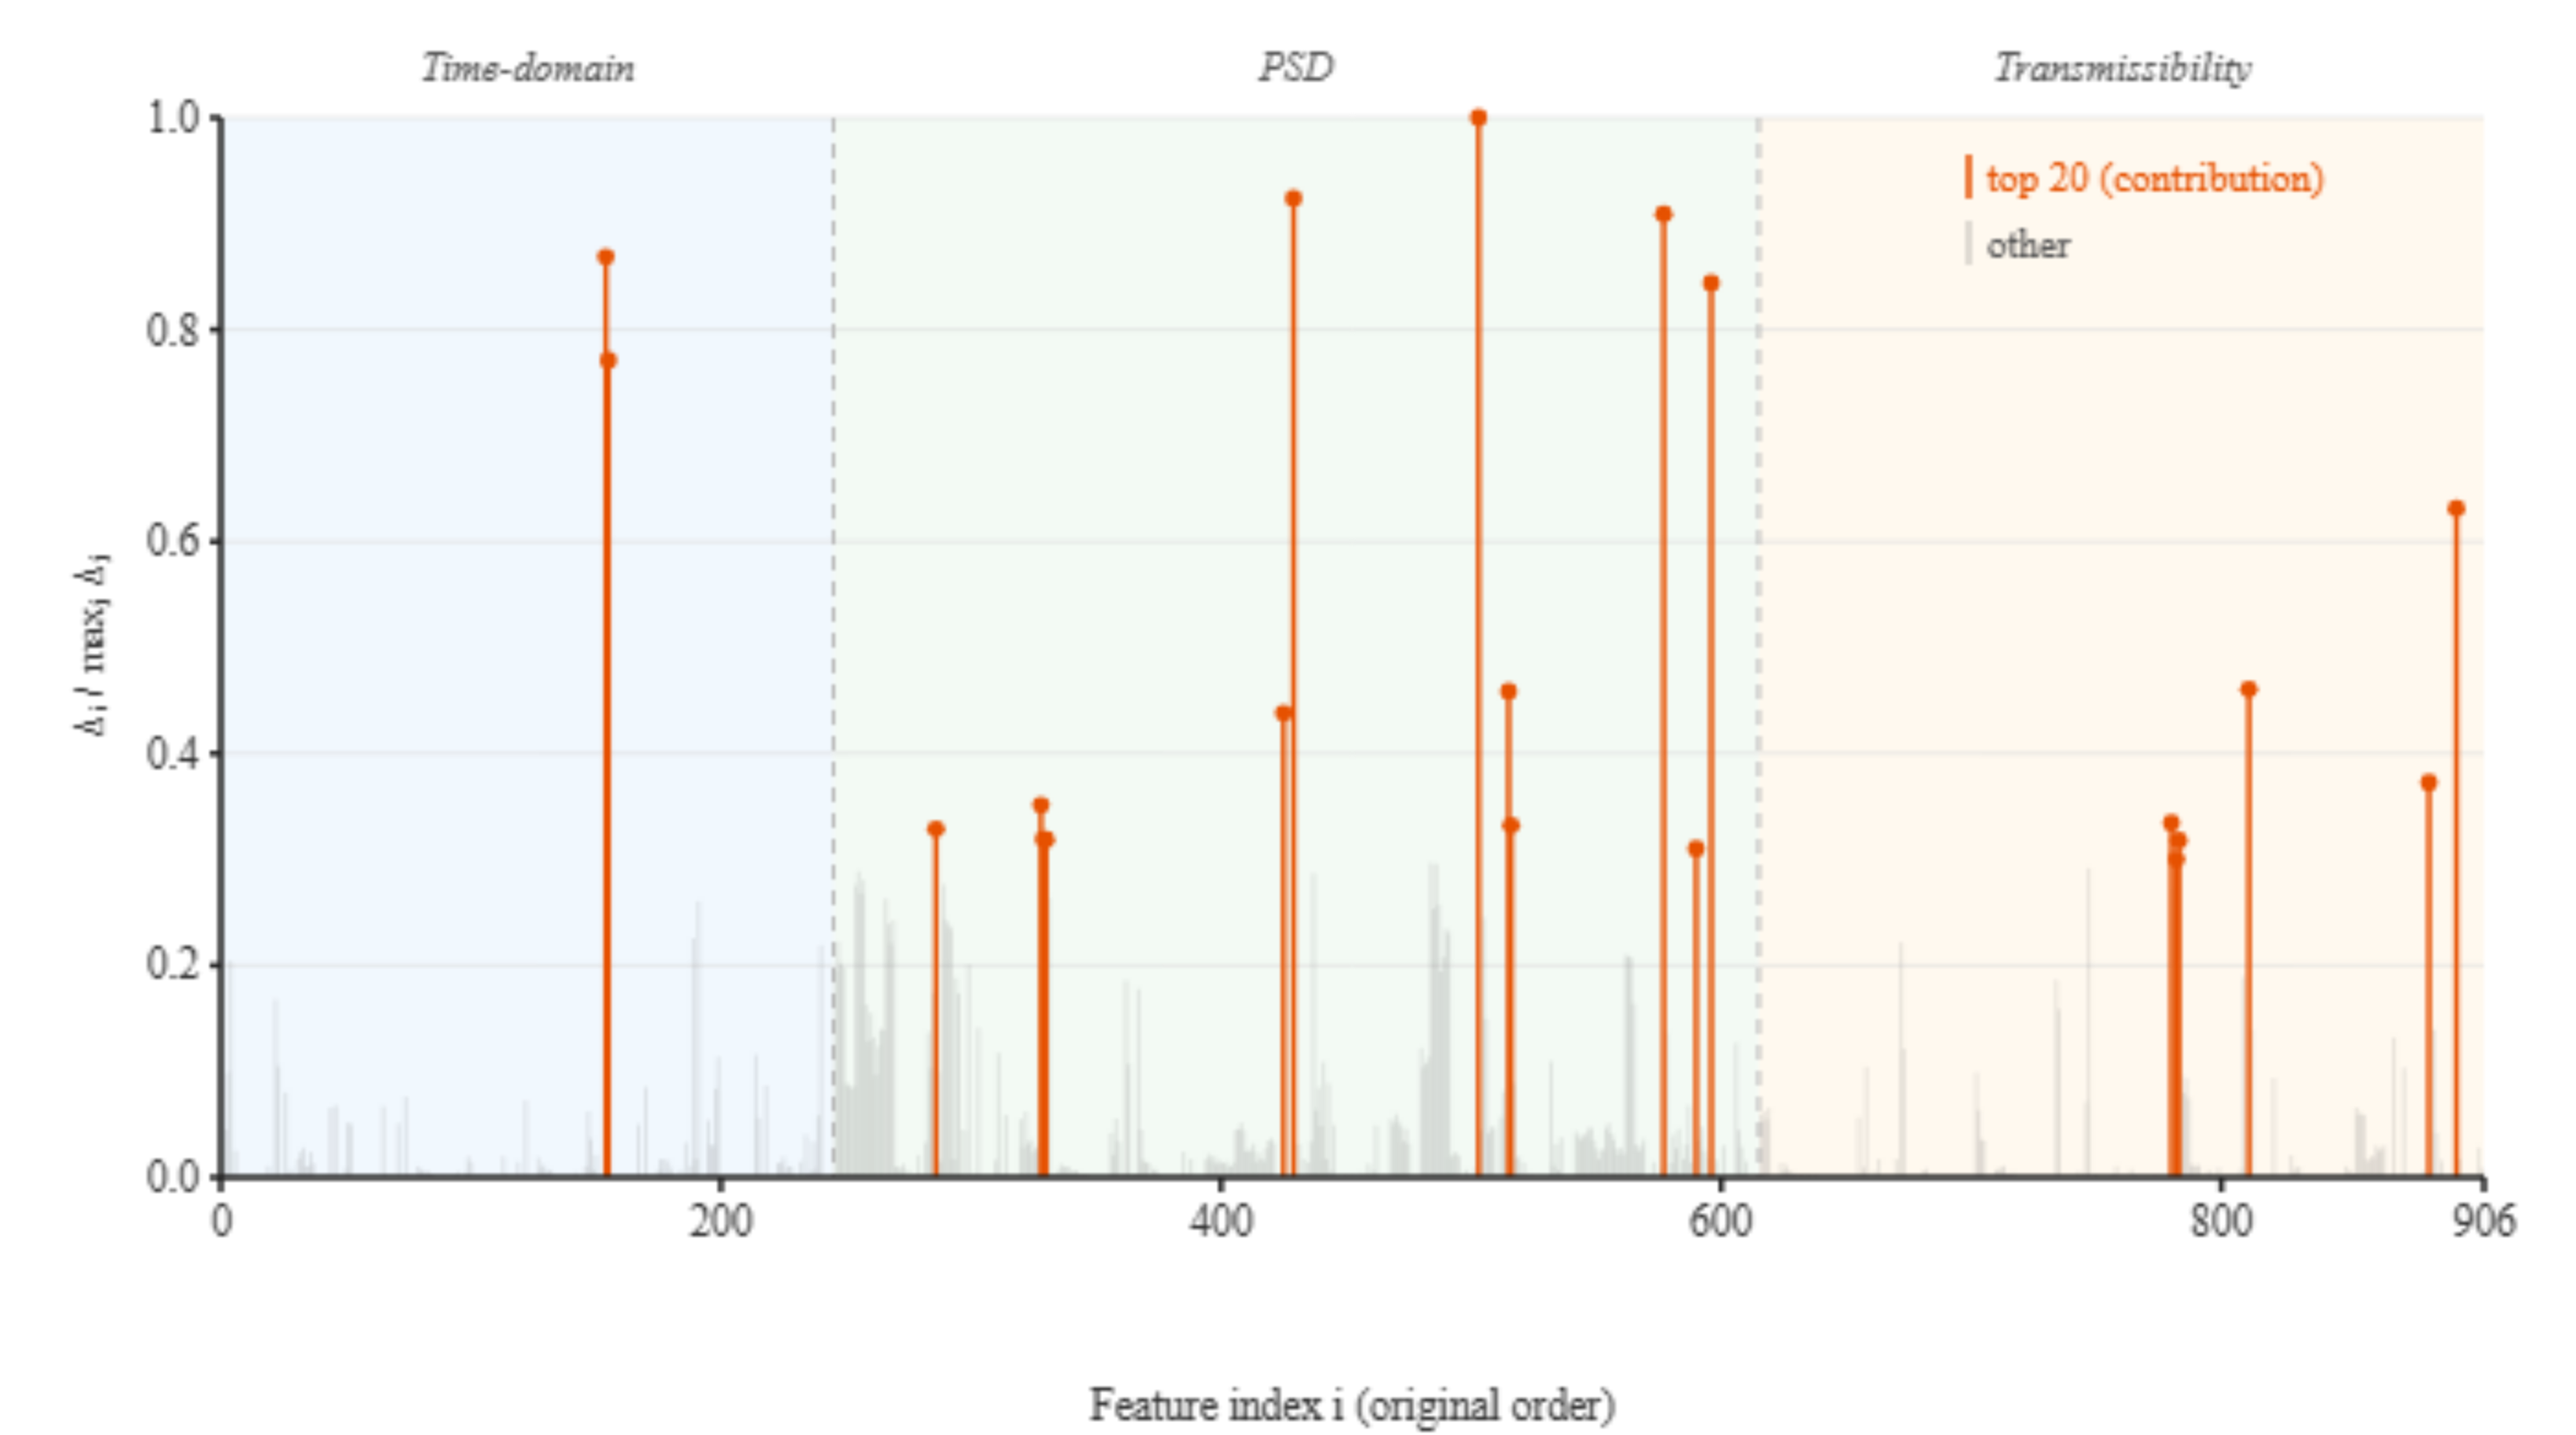
\includegraphics[width=\linewidth]{fig6.png}
\caption{Per-feature contribution $\Delta_i$ to the healthy--damaged score gap, in original feature order; top-20 contributors highlighted.}
\label{fig:attn}
\end{figure}

\begin{table}[htbp]
\centering
\caption{Top-20 physics features ranked by contribution to the mean healthy--damaged score gap.}
\label{tab:top20}
\small
\begin{tabular}{@{}clllr@{}}
\toprule
\textbf{Rank} & \textbf{Block} & \textbf{Channel} & \textbf{Descriptor} & \textbf{\% of gap} \\
\midrule
1  & PSD   & R2V     & peak-index rank 3 of 4 (by prominence)      & 3.03\% \\
2  & PSD   & R2T     & peak-index rank 3 of 4 (by prominence)      & 2.80\% \\
3  & PSD   & R3V     & peak-index rank 3 of 4 (by prominence)      & 2.76\% \\
4  & TD    & R2V     & coefficient of variation                    & 2.64\% \\
5  & PSD   & R3V     & sub-band peak height, 22.5--25.0~Hz          & 2.56\% \\
6  & TD    & R2V     & fraction of zero-valued samples              & 2.34\% \\
7  & TRANS & R3V/R1V & sub-band peak height, 27.5--30.0~Hz          & 1.92\% \\
8  & TRANS & R2V/R1V & sub-band peak height, 5.0--7.5~Hz            & 1.40\% \\
9  & PSD   & R2V     & sub-band peak height, 5.0--7.5~Hz            & 1.39\% \\
10 & PSD   & R2T     & piecewise-cubic linear term (segment 6/6)    & 1.33\% \\
11 & TRANS & R3V/R1V & sub-band peak height, 0.0--2.5~Hz            & 1.13\% \\
12 & PSD   & R2L     & std.\ of peak height                        & 1.07\% \\
13 & TRANS & R2V/R1V & piecewise-cubic constant term (segment 2/6)  & 1.01\% \\
14 & PSD   & R2V     & sub-band peak height, 7.5--10.0~Hz           & 1.01\% \\
15 & PSD   & R1V     & sharp-peak position, rank 4                  & 1.00\% \\
16 & PSD   & R2L     & piecewise-cubic cubic term (segment 1/6)     & 0.97\% \\
17 & PSD   & R2L     & piecewise-cubic quadratic term (segment 1/6) & 0.97\% \\
18 & TRANS & R2V/R1V & piecewise-cubic linear term (segment 3/6)    & 0.96\% \\
19 & PSD   & R3V     & sub-band peak height, 7.5--10.0~Hz           & 0.94\% \\
20 & TRANS & R2V/R1V & piecewise-cubic quadratic term (segment 3/6) & 0.91\% \\
\bottomrule
\end{tabular}
\end{table}

Figure~\ref{fig:profile} shows, feature by feature, why the plain score fails on
these residuals while attention succeeds. In both panels the 906
features are sorted by descending attention weight, and the two curves show
the mean squared residual over healthy and over damaged windows. Without
weighting (panel~a), the two curves track each other across the entire bank: a
healthy--damaged gap exists but is diffuse, and the coordinates dominated by
environmental variability fluctuate strongly in \emph{both} classes, so
summing all 906 coordinates equally drowns the signal---the visual
counterpart of AE-plain's AUC of $0.646$. After weighting (panel~b), the
damaged curve rises clearly above the healthy one on the high-weight features
(rank $\lesssim 500$), while the low-weight tail (rank $\gtrsim 550$) is
pressed toward zero for both classes. Because the anomaly score is
$s(x)=\sum_i a_i r_i^2$, the area between the two curves in panel~(b) is
precisely the mean score gap that detection relies on. The flat segment at the
far left of panel~(b) is the small group of constant coordinates noted earlier:
maximal weight, zero contribution. Attention does not pick out damage-sensitive
features; without labels it cannot. Instead, by trusting the coordinates that are
stable in the healthy state, it makes damage-induced deviations stand out against
a quiet background.

\begin{figure}[htbp]
\centering
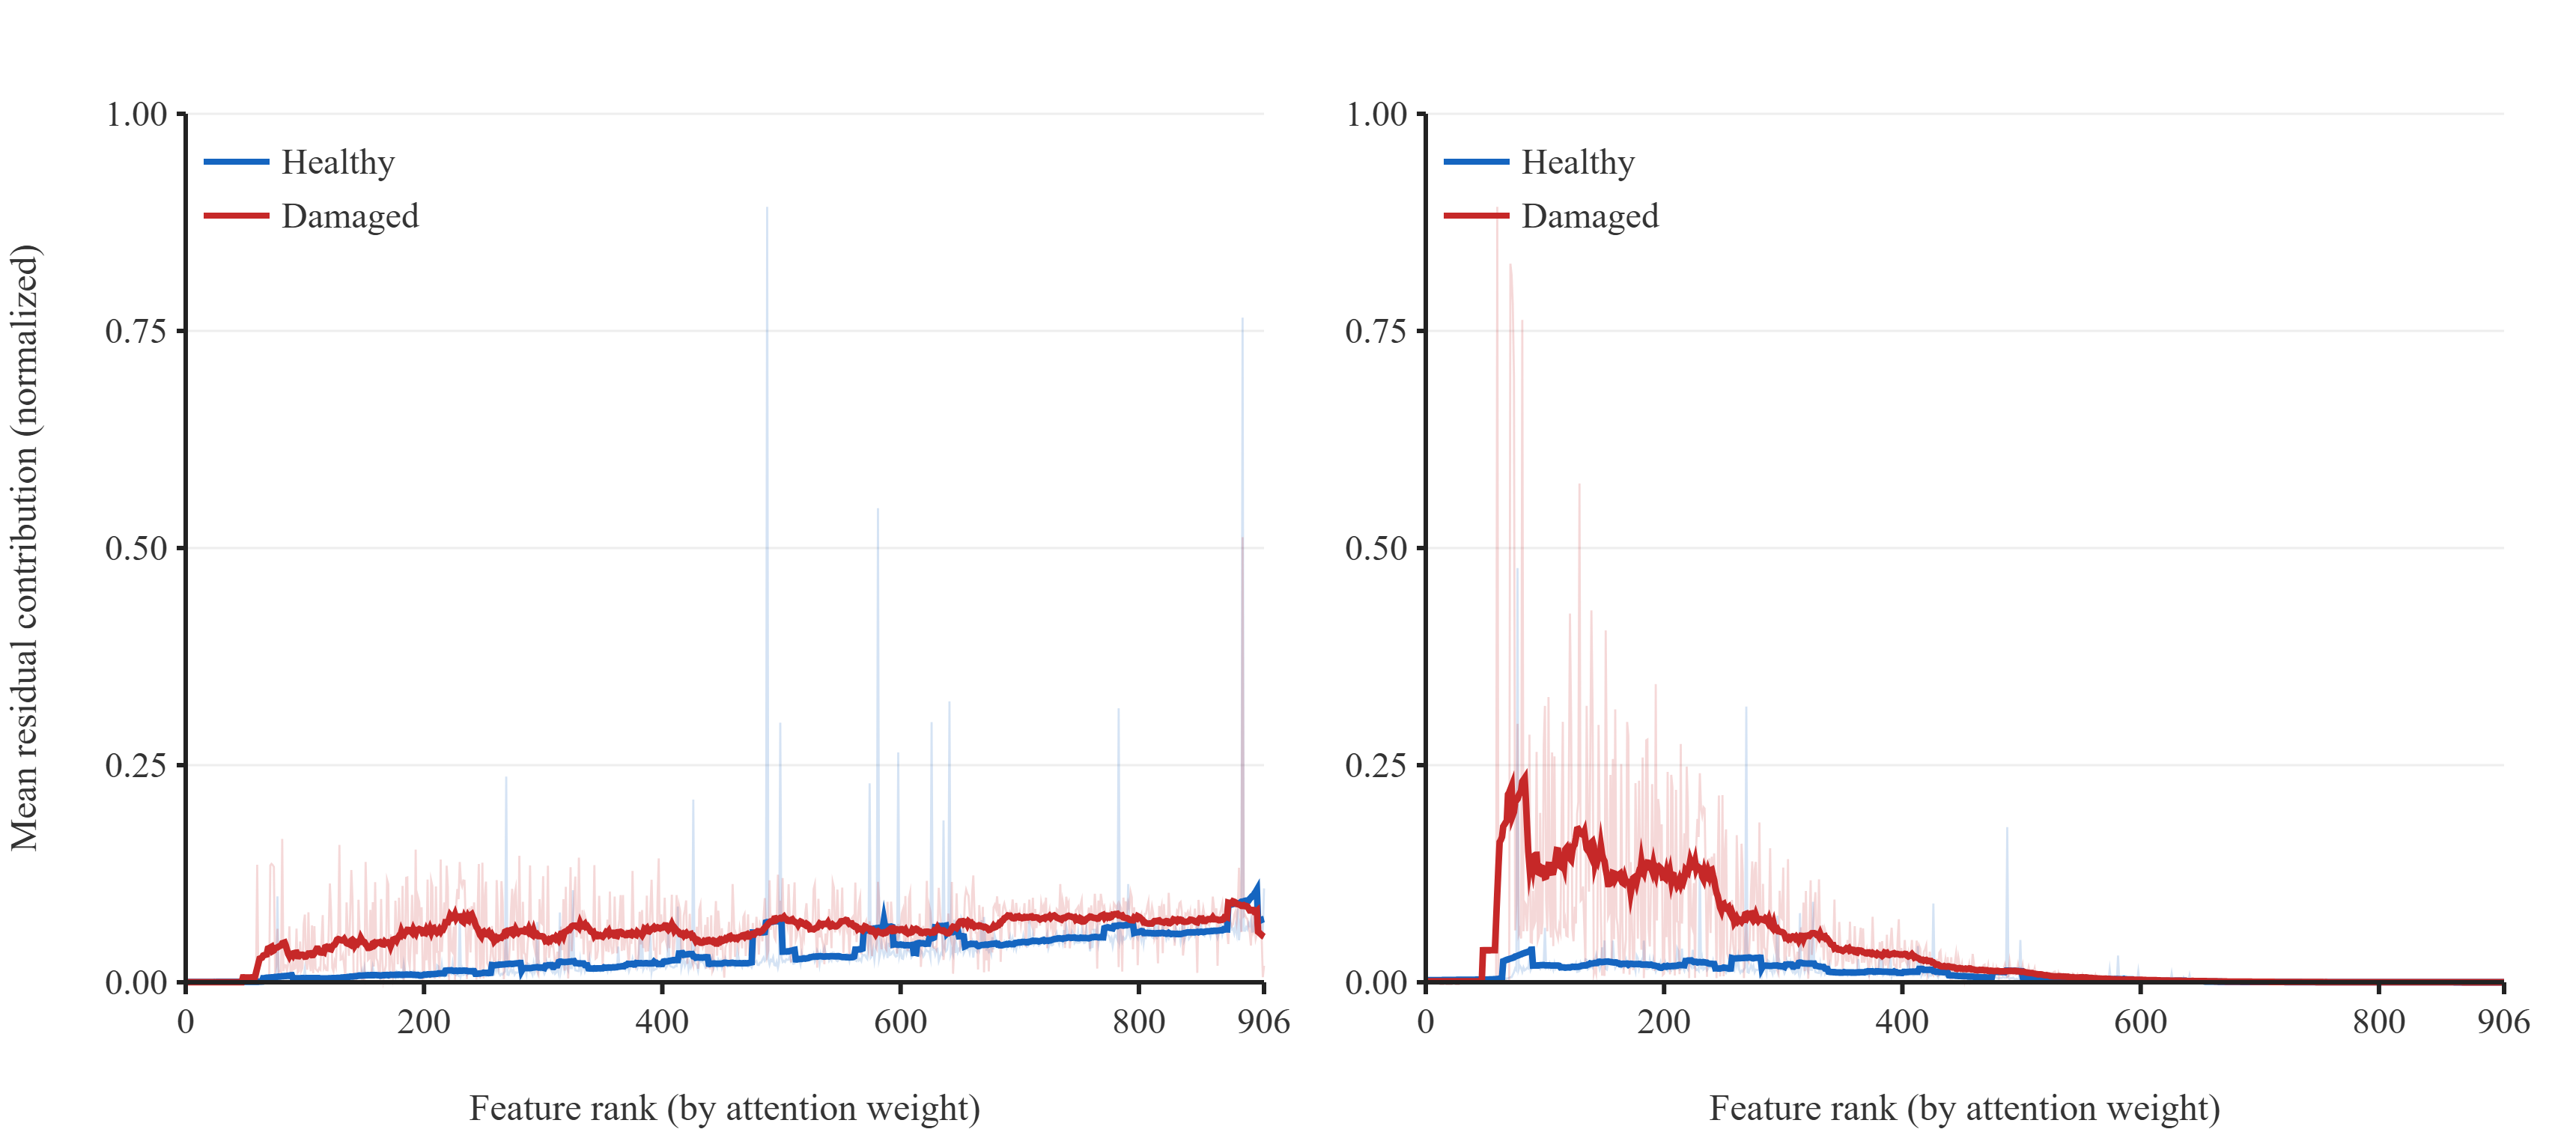
\includegraphics[width=\linewidth]{fig7.png}
\caption{Class-mean squared residuals per feature, features ordered by descending attention weight; each panel is normalized to its own maximum. (a)~Unweighted $\overline{r_i^2}$: healthy and damaged nearly coincide. (b)~Attention-weighted $a_i\,\overline{r_i^2}$: separation concentrates on the high-weight features while the noisy tail is suppressed.}
\label{fig:profile}
\end{figure}

Two simpler one-class alternatives might replace the attention stage: a
standard unsupervised detector on the full bank, and a hand-selected feature
family. Neither proves adequate. A standard unsupervised detector does not help:
an elliptic envelope on the leading principal components is no better than chance
(AUC $0.33$--$0.51$ for $3$ to $64$ components), and a Mahalanobis distance over
all features reaches only $0.681$---barely above the plain autoencoder ($0.646$)
and far below attention ($0.802$ on this run). These methods trust the
highest-variance directions of the data;
\textcolor{red}{here those directions are dominated by sources other than
damage---environmental and operational variability among them, but also
sensor noise and nonlinear response \cite{farrar2007}---consistent with
Section~\ref{sec:baselines}, where a residual-space alternative to leading
principal components (PCA squared prediction error) also underperforms
attention.}

The 906 features also fall into three physically meaningful blocks: time-domain
statistics, PSD shape descriptors, and transmissibility descriptors. A long
tradition in SHM selects one such family a priori---natural frequencies, mode
shapes, curvature, modal strain energy---and stakes performance on that choice.
Table~\ref{tab:blocks} tests that strategy directly, by restricting the
attention-weighted score to each block in turn.
\textcolor{red}{The attention weights and $\beta$ are fit once, over the full
$906$-feature bank, exactly as in Section~\ref{sec:mechanism}; each row of
Table~\ref{tab:blocks} sums the same weighted residuals over a different
subset of coordinates, rather than re-fitting $\beta$ or the weights within
that block alone.}

\begin{table}[htbp]
\centering
\caption{Detection AUC restricted to a single physics block vs.\ full-bank attention.}
\label{tab:blocks}
\small
\begin{tabular}{@{}lc@{}}
\toprule
\textbf{Feature block used for scoring} & \textbf{AUC} \\
\midrule
Time-domain statistics only                    & 0.682 \\
Transmissibility descriptors only              & 0.771 \\
PSD shape descriptors only                     & 0.783 \\
\midrule
\textbf{Attention over the full 906-feature bank (PGAE-A)} & \textbf{0.802} \\
\bottomrule
\end{tabular}
\end{table}

Every single hand-chosen block underperforms attention over the full bank, and
the ranking is not the one an expert would necessarily have predicted: on this
structure the PSD descriptors carry the most one-class signal ($0.783$),
ahead of the transmissibility descriptors ($0.771$), even though transmissibility
is classically motivated as a differential damage indicator \cite{johnson2002},
and well ahead of the time-domain statistics ($0.682$). Committing in advance to
any one family therefore forfeits performance. Attention does not simply
rediscover the best block; it integrates the reliable coordinates of several
blocks and exceeds each of them individually.

This supports a concrete methodological recommendation. Rather than searching
for the few features presumed to be damage-sensitive, generate a large and
deliberately redundant bank of physics-derived descriptors, and let a one-class
mechanism weight them from healthy data. The procedure is automatic, requires no
expert commitment to a particular physical quantity, achieves better detection
than any single family, and---unlike supervised selection---never leaves the
one-class setting.

The effect of the mechanism is visible directly in the anomaly scores.
Figure~\ref{fig:control} plots them sequentially across all
612 windows. Under
AE-plain (upper panel), scores fluctuate widely in both healthy and damaged
states: the 95th-percentile healthy threshold is regularly breached in healthy
windows and inconsistently exceeded in damaged ones, reflecting the
noise-dominated AUC of 0.646. PGAE-A (lower panel) keeps most healthy scores low
across the eight healthy states and lifts them from S9 onward, with a clear step
change at the onset of damage; a few healthy windows still spike and some damaged
windows stay low, consistent with the AUC of $0.802$. The marginal
score distributions (Figure~\ref{fig:kde}) exhibit the same effect: under plain
scoring (panel a) the healthy and damaged populations overlap broadly, whereas
under attention (panel b) the healthy scores collapse into a tight low-value
cluster and the damaged scores shift markedly higher.

\begin{figure}[htbp]
\centering
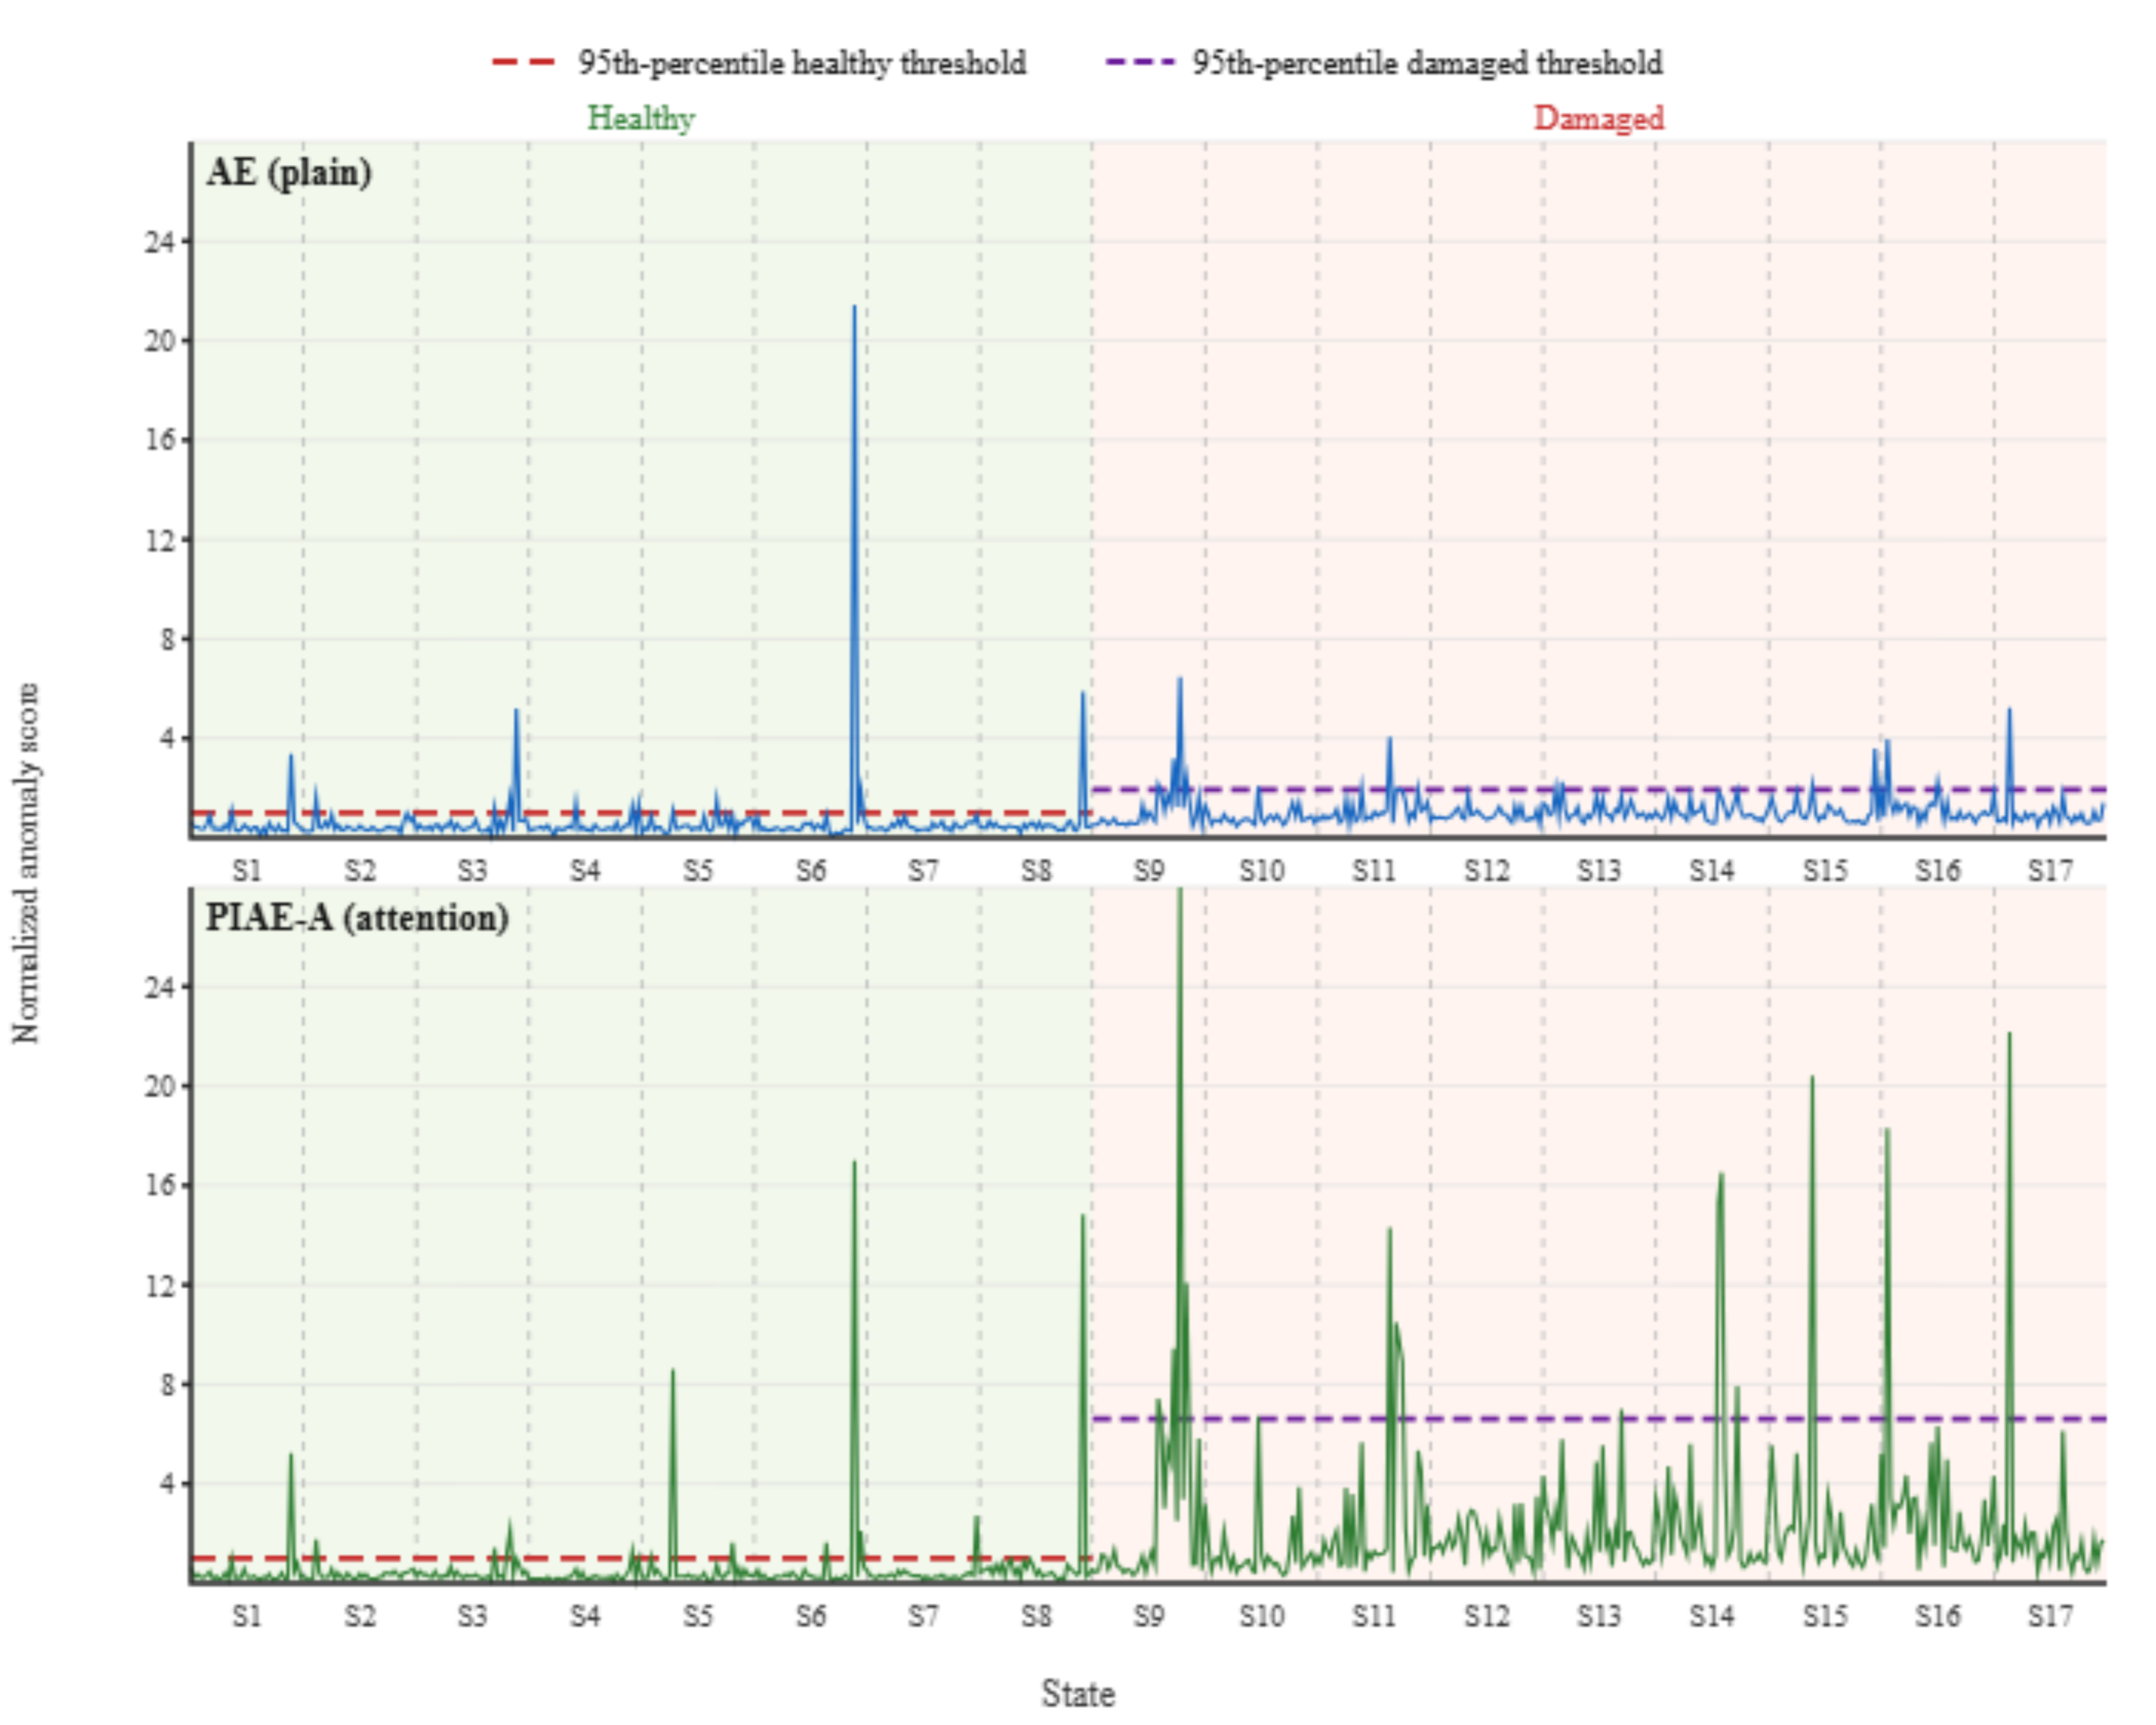
\includegraphics[width=\linewidth]{fig8.png}
\caption{Sequential anomaly scores across the 17 states\textcolor{red}{. The dashed healthy line marks the 95th-percentile alarm threshold used by the detector (Section~\ref{sec:train}); the dashed damaged line is a descriptive reference computed after the fact from the damaged scores themselves and is not part of the detection rule. Within each healthy state, the darker green band marks the windows never used to train the autoencoder.}}
\label{fig:control}
\end{figure}

\begin{figure}[htbp]
\centering
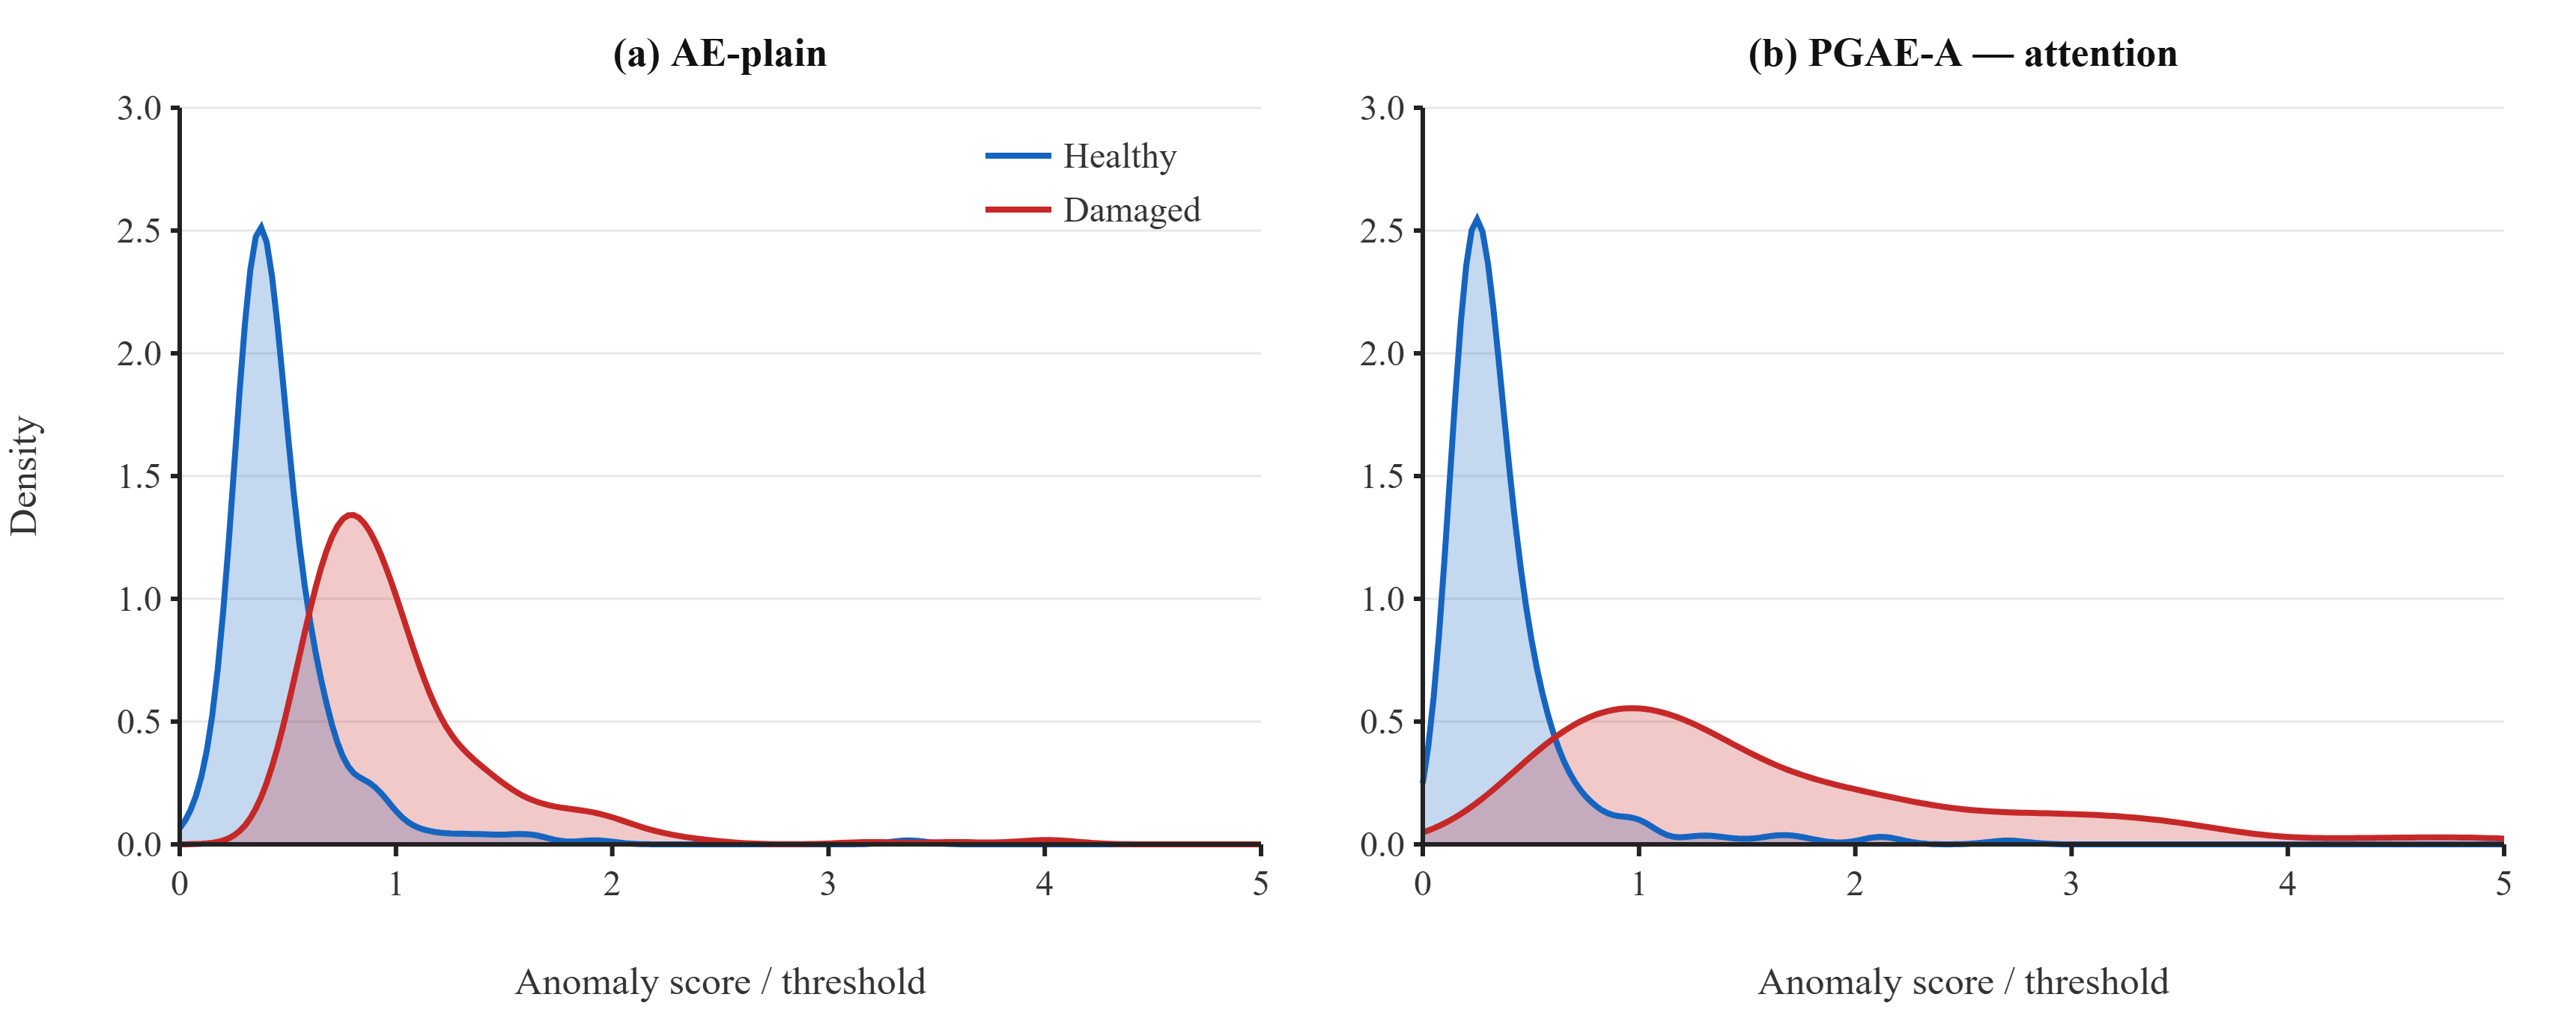
\includegraphics[width=\linewidth]{fig9.png}
\caption{Anomaly-score densities, healthy vs.\ damaged. Each score is shown relative to its own $95$th-percentile healthy alarm threshold. (a)~AE-plain, AUC~$=0.646$. (b)~PGAE-A, AUC~$=0.802$.}
\label{fig:kde}
\end{figure}

\subsection{Statistical validation}
\label{sec:main}
The preceding analyses come from a single representative run. This subsection
reports the statistics over ten independent runs---mean and standard
deviation---that underpin every claim of improvement in this paper. Reported
AUCs carry two independent sources of uncertainty, which we treat separately.

The first, \emph{training stochasticity}, reflects random weight initialization
and the random healthy train/validation split. We repeat the entire one-class
pipeline over $n=10$ independent runs, each varying both, and report the mean,
standard deviation and a $95\%$ Student-$t$ interval. The number of runs needed
for a target confidence half-width $\delta$ follows from
\begin{equation}
n \;\ge\; \left(\frac{t_{n-1,\,0.975}\;\hat\sigma_{\mathrm{run}}}{\delta}\right)^{\!2};
\label{eq:seedn}
\end{equation}
with the observed $\hat\sigma_{\mathrm{run}}\approx0.014$, ten runs give
$\delta\approx0.01$. For the specific claim that PGAE-A improves on the plain
autoencoder, a power analysis is more relevant: because the two detectors share
the trained network and test windows, we use a paired test, and the observed
effect ($\approx0.15$ AUC) is roughly ten times $\sigma_{\mathrm{run}}$; the
minimum detectable sample size
\begin{equation}
n \;\ge\; \left(\frac{(z_{1-\alpha/2}+z_{1-\beta_{\mathrm{pow}}})\,\sigma_\Delta}{\Delta}\right)^{\!2}
\label{eq:powern}
\end{equation}
evaluates to fewer than 3 runs at $99\%$ power, so ten runs are ample.

The second, \emph{finite-test uncertainty}, arises from estimating AUC on a
limited test set and does \emph{not} shrink with more runs. By the Hanley--McNeil estimator
\cite{hanley1982}, the standard error of $\widehat{\mathrm{AUC}}$ is
\begin{equation}
\begin{split}
\mathrm{SE}\!\left(\widehat{\mathrm{AUC}}\right)
&\;=\; \sqrt{\frac{A(1-A)+(n_D-1)(Q_1-A^2)+(n_H-1)(Q_2-A^2)}{n_D\,n_H}},\\[4pt]
&\quad Q_1=\frac{A}{2-A},\qquad Q_2=\frac{2A^2}{1+A}.
\end{split}
\label{eq:hmse}
\end{equation}
At $\mathrm{AUC}=0.80$ with $n_D=324$ damaged and $n_H=32$ healthy test windows,
Eq.~\eqref{eq:hmse} gives $\mathrm{SE}\approx0.033$. This exceeds the
between-run standard deviation: the binding constraint is the small healthy
test set, not the number of training runs---a point we return to below. All results
report both quantities.

We now report the multi-run detection performance of the three detectors.
Table~\ref{tab:main} lists them together with their inputs, label usage, and
mean ROC-AUC on the Z24 benchmark.
\emph{AE-plain} is the autoencoder backbone with uniform scoring
$s(x)=\sum_i r_i^2$---the natural one-class baseline over the same feature
bank. \emph{PGAE-A} adds the unsupervised feature attention. The
\emph{elliptic envelope} is a Mahalanobis
outlier detector trained on the four features selected by a gradient-boosted
classifier with damage labels \cite{abdrabo2024}; it violates the one-class
constraint and is included as an upper reference only.
\textcolor{red}{Its run-to-run variation in Table~\ref{tab:main} has the same
source as the one-class detectors': the mean and covariance it is fit to
are computed from the same random $80/20$ healthy split used to train the
autoencoder at each seed, not from any property specific to the elliptic
envelope itself.}

\begin{table}[htbp]
\centering
\caption{Detection performance on Z24. ``Labels?'' indicates whether damage labels enter anywhere in the pipeline.}
\label{tab:main}
\small
\begin{tabular}{@{}llcc@{}}
\toprule
\textbf{Detector} & \textbf{Input} & \textbf{Labels?} &
\textbf{AUC (mean $\pm$ std)} \\
\midrule
AE-plain (plain scoring)  & 906 physics features & no  & $0.643 \pm 0.007$ \\
\textbf{PGAE-A (ours)}  & 906 physics features & \textbf{no} &
$\mathbf{0.795 \pm 0.014}$ \\
\midrule
Elliptic envelope       & 4 label-selected features & yes & $0.944 \pm 0.002$ \\
\bottomrule
\end{tabular}
\end{table}

Statistics are over ten independent runs as described above. The two one-class
detectors share the same autoencoder, the same feature bank and the same
one-class rule for $\beta$, and differ only in how per-feature residuals are
combined into an anomaly score. The automatic rule for $\beta$ is itself stable
across runs, selecting a nearly constant effective retention
$\alpha = 0.31 \pm 0.005$ ($\beta = 0.065 \pm 0.007$) without any target being
specified. Unsupervised attention raises AUC from
$0.643 \pm 0.007$ to $0.795 \pm 0.014$ (Figure~\ref{fig:roc}); the paired
improvement is
$0.151 \pm 0.015$ ($p = 1.2\times10^{-10}$, paired $t$-test), an effect roughly
an order of magnitude larger than the run-to-run variation. Consistent with
the uncertainty analysis above, the between-run standard deviation ($0.014$) is smaller than
the Hanley--McNeil finite-test standard error ($0.033$): the dominant
uncertainty is the small healthy test set, not the training runs, so
additional runs would not narrow the estimate further. The supervised
reference remains ahead at $0.944$.
\textcolor{red}{This should be read as a supervised comparison rather than an
isolated measure of what damage labels are worth: the elliptic envelope
differs from PGAE-A not only in using labels, but also in feature
dimensionality ($4$ label-selected features versus the full $906$-feature
bank) and detector formulation (Mahalanobis distance versus an autoencoder
with attention-weighted residuals), so the gap reflects all of these choices
together, not damage labels alone.}

\textcolor{red}{The healthy training pool draws from only eight structural
states, so the random $80/20$ split used above can place windows from the
same state in both the training and validation portions. Replacing it with
leave-one-state-out validation, where each state is held out in turn, gives
a mean AUC of $0.780 \pm 0.012$ across the eight folds, compared with
$0.795 \pm 0.014$ under the random split---a modest but measurable
difference (Welch $t$-test, $p=0.031$). Even the weakest fold, $0.762$,
remains far above AE-plain's $0.643$. Supplementary Material S4 reports the
result for each held-out state. This sensitivity to how little healthy data
is available per state echoes recent work on short-term damage alarming
with limited vibration data \cite{entezami2024measurement}.}

\textcolor{red}{The Hanley--McNeil standard error above also assumes the test windows are
independent, but the $324$ damaged windows come from only nine states and
the $32$ healthy test-pool windows from eight, and windows from the same
state are correlated. We instead estimate the sampling distribution of AUC
with a cluster bootstrap that resamples states, not individual windows, with
replacement. This gives a standard error of $0.049$ and a $95\%$ interval of
$[0.705, 0.895]$, both wider than the Hanley--McNeil value of $0.032$.
Supplementary Material S5 reports the full comparison, including a
window-level bootstrap that ignores the state structure for reference.}

\textcolor{red}{ROC-AUC is threshold-free; at the specific $95$th-percentile
healthy alarm threshold used throughout this section, the detector attains a
sensitivity of $0.289 \pm 0.164$ and a specificity of $0.875 \pm 0.021$ on the
held-out evaluation set, for a balanced accuracy of $0.582 \pm 0.079$. The
observed false-alarm rate, $0.125 \pm 0.021$, exceeds the $5\%$ design
target because it is measured on the genuinely held-out healthy test-pool
windows rather than on the validation-normal data the threshold is
calibrated from. Sensitivity at this conservative operating point is
modest---correctly flagging roughly three in ten damaged windows without
exceeding the healthy false-alarm budget---which is why ROC-AUC, not tied
to any single threshold, remains the primary metric for this comparison.}

\begin{figure}[htbp]
\centering
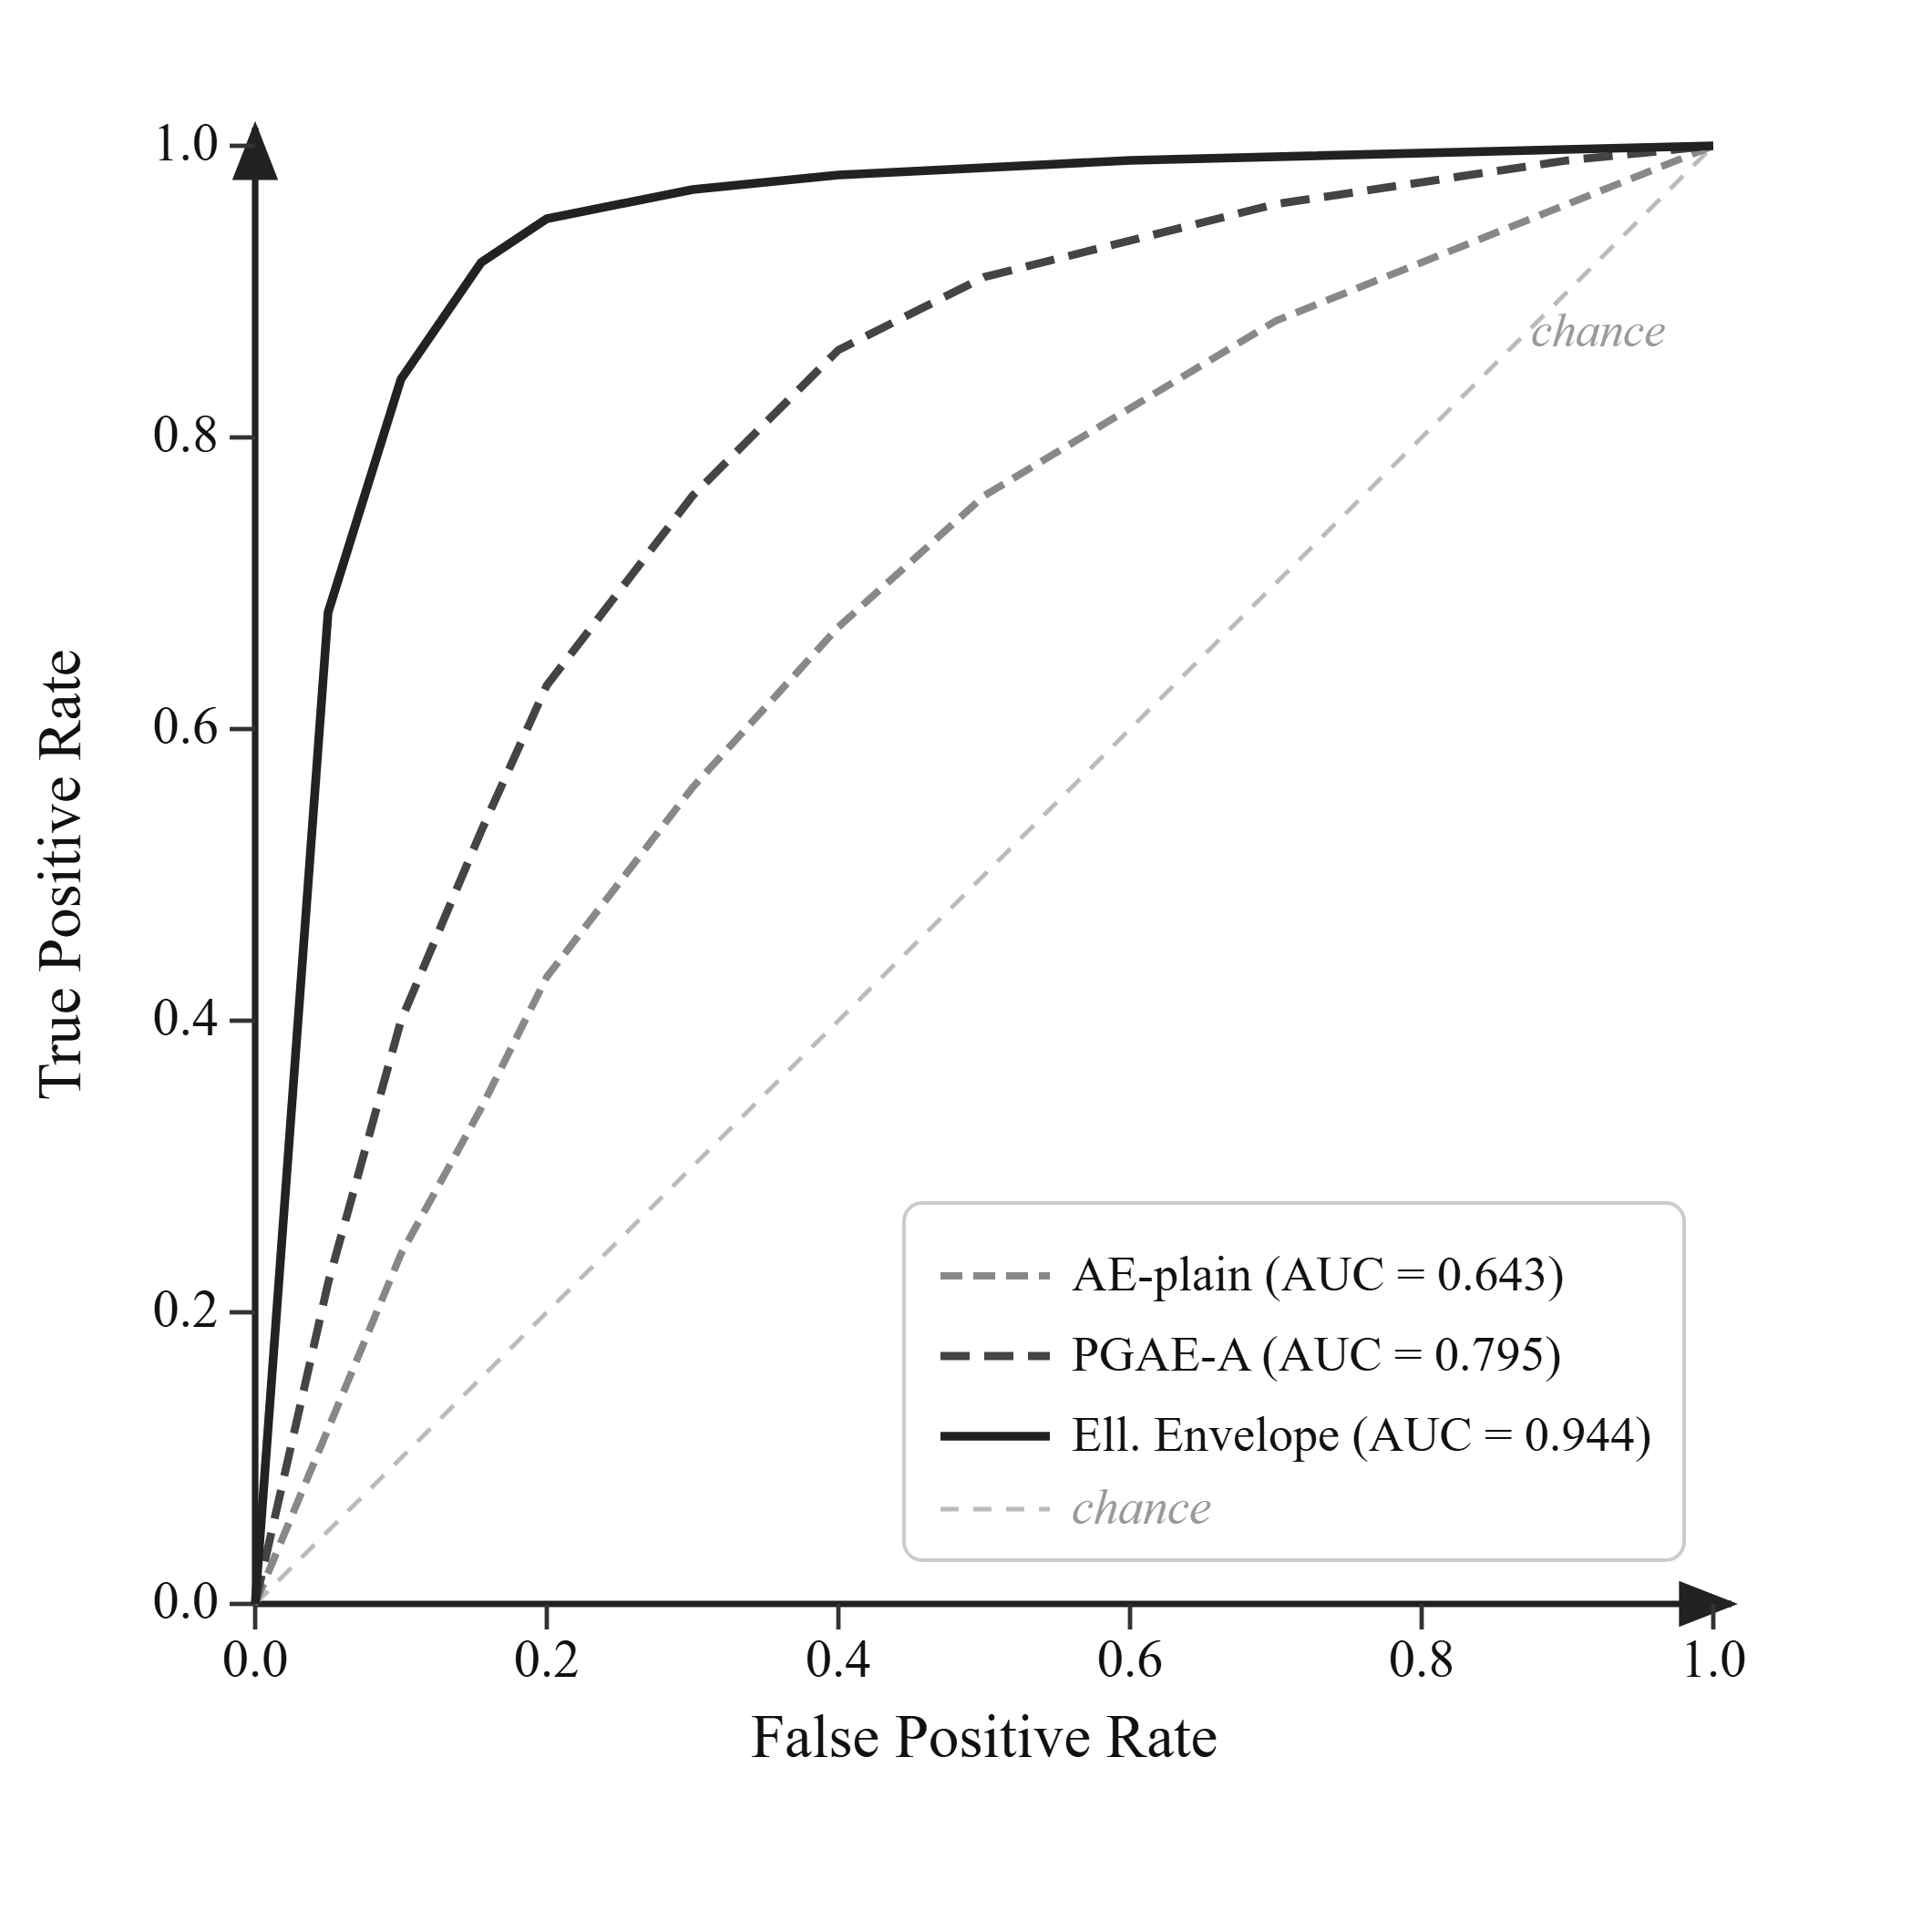
\includegraphics[width=0.75\linewidth]{fig10.png}
\caption{ROC curves for the three detectors at their mean AUC.}
\label{fig:roc}
\end{figure}

\FloatBarrier
% =====================================================================
% NEW SUBSECTION — round-1 revision, response to Reviewer 1 #4 / Reviewer 2 #3
% =====================================================================
\color{red}

\subsection{Sensitivity to the healthy-state definition}
\label{sec:settlement}

Four of the eight healthy states, S4--S7, are pier settlements of $20$--$95$~mm
(Table~\ref{tab:states}). Under the benchmark's own convention these are
treated as healthy, since the settlement is later reversed. This convention
raises a natural concern: training the autoencoder on these settlement
states, rather than on a narrower and more strictly undamaged set, could
itself be what produces the reported detection performance. We test this
directly rather than rely on the convention alone.

The most direct test is to remove S4--S7 from the healthy training pool and
retrain. Doing so, however, creates a complication. Removing four of the
eight states also removes half of the available healthy training data, so a
drop in performance could then mean two different things: that the
settlement states specifically matter, or simply that the autoencoder had
less data to learn from. To tell these explanations apart, we add a third,
control condition: a random subsample of the original training pool, cut
down to the same reduced size, but with all eight healthy states still
represented. Comparing this control against the settlement-excluded run
isolates the effect of the settlement states themselves, with the amount of
training data held fixed. All three conditions are scored on the same
evaluation set and the same ten-seed protocol as Table~\ref{tab:main}.

Table~\ref{tab:settlement} summarizes the result. Training on the full
healthy pool of $256$ windows, the original protocol, reaches an AUC of
$0.795$. Reducing the pool to $128$ windows while still drawing from all
eight states lowers AUC only modestly, to $0.762$, a cost attributable to
training on less data. Removing the settlement states specifically, at that
same reduced size, lowers AUC much further, to $0.632$, and does so
consistently: in every one of the ten seeds, the model trained without the
settlement states scores below the size-matched model trained with them
included. The settlement states therefore account for most of the difference
between the original protocol and a model trained without them; the reduced
amount of training data explains only a small part of it.

Table~\ref{tab:perstate} breaks the same result down by individual state.
Among the eight healthy states, S6, an $80$~mm settlement, and S8, the
post-restoration reference, receive the highest and most variable scores.
This pattern is worth checking, since it is what one would expect if the
autoencoder were partly confusing settlement with damage. It does not change
the overall separation, however: both states still score below every one of
the nine damaged states.

Taken together, these results support two conclusions. The settlement states
are not a source of error: the model does not mistake them for damage, in
aggregate or individually. At the same time, they are not incidental to the
reported performance: the diversity of the healthy training pool, and
specifically the inclusion of pier settlements up to $95$~mm, accounts for
most of the detection accuracy reported in Table~\ref{tab:main}.

\begin{table}[htbp]
\color{red}
\centering
\captionsetup{labelfont={color=red},font={color=red}}
\caption{Detection AUC under three healthy training-pool compositions (ten
seeds each; evaluation set unchanged across rows).}
\label{tab:settlement}
\small
\begin{tabular}{@{}lccc@{}}
\toprule
\textbf{Training-pool composition} & $N_{\text{healthy}}$ & \textbf{States used} & \textbf{AUC (mean $\pm$ std)} \\
\midrule
Full (original protocol)           & 256 & S1--S8      & $0.795 \pm 0.014$ \\
Matched random subsample           & 128 & S1--S8      & $0.762 \pm 0.017$ \\
Excl.\ settlement (S4--S7 removed) & 128 & S1--S3, S8  & $0.632 \pm 0.011$ \\
\bottomrule
\end{tabular}
\end{table}

\begin{table}[htbp]
\color{red}
\centering
\captionsetup{labelfont={color=red},font={color=red}}
\caption{Attention-weighted anomaly score by state (Full-protocol model,
mean $\pm$ std over ten seeds).}
\label{tab:perstate}
\small
\begin{tabular}{@{}clc@{}}
\toprule
\textbf{State} & \textbf{Condition} & \textbf{Score (mean $\pm$ std)} \\
\midrule
S1  & Undamaged reference                     & $0.089 \pm 0.159$ \\
S2  & Reference (settlement system installed) & $0.065 \pm 0.028$ \\
S3  & Reference measurement                   & $0.098 \pm 0.129$ \\
S4  & Pier settlement, 20~mm                  & $0.064 \pm 0.065$ \\
S5  & Pier settlement, 40~mm                  & $0.093 \pm 0.145$ \\
S6  & Pier settlement, 80~mm                  & $0.157 \pm 0.420$ \\
S7  & Pier settlement, 95~mm                  & $0.063 \pm 0.071$ \\
S8  & Pier lifted; new reference               & $0.162 \pm 0.448$ \\
\midrule
S9  & Concrete spalling, 12~m$^2$             & $0.588 \pm 1.089$ \\
S10 & Concrete spalling, 24~m$^2$             & $0.199 \pm 0.190$ \\
S11 & Landslide at abutment                   & $0.455 \pm 0.548$ \\
S12 & Failure of a concrete hinge             & $0.274 \pm 0.128$ \\
S13 & Failure of 2 anchor heads               & $0.344 \pm 0.256$ \\
S14 & Failure of 4 anchor heads               & $0.449 \pm 0.560$ \\
S15 & Rupture of 54 tendon wires               & $0.396 \pm 0.517$ \\
S16 & Rupture of 100 tendon wires              & $0.482 \pm 0.475$ \\
S17 & Rupture of 154 tendon wires              & $0.342 \pm 0.586$ \\
\bottomrule
\end{tabular}
\end{table}

\FloatBarrier

% =====================================================================
% NEW SUBSECTION — round-1 revision, response to Reviewer 1 #5 / #6, Reviewer 2 #15
% =====================================================================

\subsection{Comparison with alternative one-class baselines}
\label{sec:baselines}

Up to this point, PGAE-A has been evaluated against a plain autoencoder using
the same feature bank, as well as a supervised reference model utilizing
damage labels. In this section, we further compare it against five
established one-class methods. To ensure a fair comparison, each method is
trained on the same pool of $256$ healthy windows and evaluated on the
identical test set of $324$ damaged and $32$ healthy windows, following the
ten-seed protocol established in Table~\ref{tab:main}.

These five alternative methods are detailed below in ascending order of
their AUC, mirroring their sequence in Table~\ref{tab:baselines}. The first
method, a One-Class SVM with a radial basis function kernel, serves as a
general-purpose one-class detector applied directly to the standardized
$906$-feature bank, completely independent of the autoencoder. The second
method, PCA squared prediction error, also bypasses the autoencoder. Here,
principal component analysis is fitted to the healthy training data,
retaining the leading $32$ components to align with the autoencoder's
bottleneck dimension. Each window is then scored based on its squared
reconstruction error within the discarded residual subspace, distinct from
the leading-component Mahalanobis distance discussed in
Section~\ref{sec:mechanism}. The third and fourth alternatives utilize the
same trained autoencoder as PGAE-A but substitute the softmax attention
mechanism with a fixed weighting approach. Specifically, a MAD-normalized
score divides each squared residual by its median absolute deviation over
the healthy training split---providing a robust scale estimate against
outliers---prior to summation. A variance-normalized score applies this
exact same principle, substituting the median absolute deviation with
variance. Finally, the fifth method, Isolation Forest, acts as another
general-purpose one-class detector fitted directly to the standardized
features.
\textcolor{red}{Beyond these five, other recent one-class approaches
address related challenges under environmental and operational variability,
including manifold-learning-aided clustering with probabilistic anomaly
detection \cite{entezami2025mssp} and feature selection for unsupervised
defect detection under varying operating conditions \cite{ashkarkalaei2025};
we do not implement these directly, as they target somewhat different
problem settings, but they position the present comparison within the
broader one-class literature.}

Table~\ref{tab:baselines} presents the resulting AUCs for these five
alternatives alongside AE-plain and PGAE-A. All five fall short of PGAE-A.
Isolation Forest comes closest, but PGAE-A outperforms it on every one of the
ten identical training splits. One-Class SVM performs worst of all, even
below AE-plain, likely because its radial basis function kernel struggles to
separate the two classes in this high-dimensional, small-sample setting.

\begin{table}[htbp]
\color{red}
\centering
\captionsetup{labelfont={color=red},font={color=red}}
\caption{Detection AUC for PGAE-A and five one-class alternatives, alongside
the plain-autoencoder baseline (ten seeds; same evaluation set as
Table~\ref{tab:main}).}
\label{tab:baselines}
\small
\begin{tabular}{@{}lc@{}}
\toprule
\textbf{Method} & \textbf{AUC (mean $\pm$ std)} \\
\midrule
One-Class SVM (RBF kernel)            & $0.591 \pm 0.004$ \\
AE-plain (uniform residual weighting) & $0.643 \pm 0.007$ \\
PCA squared prediction error ($k=32$) & $0.682 \pm 0.006$ \\
MAD-normalized residual               & $0.725 \pm 0.009$ \\
Variance-normalized residual          & $0.735 \pm 0.008$ \\
Isolation Forest                      & $0.753 \pm 0.017$ \\
\textbf{PGAE-A (softmax attention, ours)} & $\mathbf{0.795 \pm 0.014}$ \\
\bottomrule
\end{tabular}
\end{table}

\FloatBarrier
\color{black}
% =====================================================================
\section{Conclusion}
\label{sec:conclusion}
Damage detection on operational structures must be a one-class
problem\textcolor{red}{, requiring no damage label at any stage.} We proposed a
physics-guided autoencoder with unsupervised feature attention (PGAE-A) that
removes this dependency. Attention weights are derived from how reliably each
physics feature is reconstructed in the healthy state, so
\textcolor{red}{the most reliably reconstructed coordinates dominate the
anomaly score and the least reliably reconstructed coordinates are
suppressed.} Using healthy data only, PGAE-A substantially improves detection over a plain
physics-feature autoencoder, without any damage label. A supervised reference
that is allowed to select features with labels remains ahead;
\textcolor{red}{because it also differs in feature dimensionality and
detector formulation, this comparison indicates the general order of what a
supervised pipeline can reach, rather than isolating the cost of the
one-class constraint alone.}

Beyond the specific model, the experiments support a change of practice. The
classical approach of committing in advance to a few putatively
damage-sensitive quantities---natural frequencies, mode shapes, curvature,
modal strain energy---is not supported by the present results: no individual
physics block matched attention over the full redundant bank, and the block
most likely to be selected on theoretical grounds was not the most informative
on this structure. Standard unsupervised subspace methods do not resolve this
difficulty either, because the leading variance directions of such feature banks
encode environmental variation rather than damage. Generating many
physics-derived features and weighting them with a one-class attention
mechanism is automatic, outperforms expert pre-selection, and remains within the
one-class setting.

Several limitations frame this work. First, a one-class detector cannot reach
the accuracy of one that is permitted to use damage labels. PGAE-A weights the
features that \textcolor{red}{are reconstructed most reliably in the healthy state}, assuming a
departure from health will show up in exactly those features. This assumption is
imperfect: a feature can be highly predictable in the healthy state yet barely
change under damage, so it receives a large weight but adds no detection signal.
Narrowing this gap without labels is the central open problem, with contrastive
or robust attention, feature self-attention, mechanics-informed priors, and
explicit EOV normalization as promising directions. Second, the estimate is
limited by the small healthy test set rather than the number of runs: the
run-to-run dispersion ($\sigma\approx0.014$) is already below the finite-test
standard error ($\approx0.033$), so a larger test set or leave-one-scenario-out
evaluation would help more than additional runs. Third, a single structure over
a short campaign limits environmental coverage; validation across structures,
seasons, and long-term monitoring---and whether attention weights transfer
between structures---is left for future work. Finally, feature extraction is fast: on a laptop
CPU the FFT-accelerated front end processes each $163.8$~s window in only about
$4.5\%$ of its duration, comfortably faster than real time. Once the attention
weights are computed from healthy data and then fixed, scoring reduces to a
simple, transparent rule light enough for on-site (edge) hardware.

\textcolor{red}{Several further limitations concern how the reported estimate
should be read. Four of the eight healthy states are pier settlements up to
$95$~mm, and the reported AUC depends materially on their presence in the
training pool: at matched training-pool size, excluding them costs roughly
thirteen points of AUC (Section~\ref{sec:settlement}). The feature bank is
deliberately redundant, so part of what the attention mechanism rewards in
any single feature may reflect correlation with other features in the bank
rather than a property specific to the healthy structure; the weights should
be read as an operational reconstruction-reliability ranking, not as
evidence of which physical quantity the structure controls. Supplementary
Material S3 tests this directly: across the non-constant features, an
independent redundancy score computed on held-out healthy data correlates
with attention weight at $\rho=0.611$, and most of the twenty most heavily
weighted features duplicate another feature in the bank almost exactly.
Windows from the
same structural state are correlated rather than independent: accounting
for this in validation (leave-one-state-out) and in the statistical analysis
(a cluster bootstrap over states) each lowers the estimate or widens its
uncertainty interval modestly, without changing the central conclusion
(Section~\ref{sec:main}; Supplementary Material S4--S5). These are
properties of the reported estimate itself, not items deferred to future
work, and a reader should weigh them alongside the headline numbers in
Table~\ref{tab:main}.}

% =====================================================================
\color{red}
\section*{Data and Code Availability}
The raw Z24
acceleration data are not redistributed here; they are available from KU
Leuven on request (\url{https://bwk.kuleuven.be/bwm/z24}). The model,
evaluation, and figure-generation code will be made public at
\url{https://github.com/chungntu/PGAE-A} upon acceptance.

\bigskip
\noindent\textbf{Supplementary Material.} A Supplementary Material document
accompanies this article, comprising Sections S1--S6: sensitivity to
constant features (S1), sensitivity to the calibration subset (S2),
sensitivity to feature redundancy (S3), leave-one-state-out validation
(S4), a cluster-bootstrap confidence interval for AUC (S5), and full
feature bank definitions (S6).
\color{black}

% =====================================================================
\section*{Acknowledgments}
This research was funded by Nha Trang University under grant number
TR2025-13-07.

% =====================================================================
\begin{thebibliography}{20}

\bibitem{farrar2007}
C.~R. Farrar, K.~Worden,
``An introduction to structural health monitoring,''
\emph{Philosophical Transactions of the Royal Society A},
365(1851):303--315, 2007.
\url{https://doi.org/10.1098/rsta.2006.1928}

\bibitem{farrar2012}
C.~R. Farrar, K.~Worden,
\emph{Structural Health Monitoring: A Machine Learning Perspective},
Wiley, Chichester, 2012.
\url{https://doi.org/10.1002/9781118443118}

\bibitem{worden2000}
K.~Worden, G.~Manson, N.~R. Fieller,
``Damage detection using outlier analysis,''
\emph{Journal of Sound and Vibration}, 229(3):647--667, 2000.
\url{https://doi.org/10.1006/jsvi.1999.2514}

\bibitem{tax2004}
D.~M.~J. Tax, R.~P.~W. Duin,
``Support vector data description,''
\emph{Machine Learning}, 54(1):45--66, 2004.
\url{https://doi.org/10.1023/B:MACH.0000008084.60811.49}

\bibitem{scholkopf1999}
B.~Sch\"olkopf, R.~C. Williamson, A.~J. Smola, J.~Shawe-Taylor, J.~C. Platt,
``Support vector method for novelty detection,''
\emph{Advances in Neural Information Processing Systems 12 (NIPS 1999)},
pp.~582--588, 1999.

\bibitem{bull2019}
L.~Bull, K.~Worden, R.~Fuentes, G.~Manson, E.~Cross, N.~Dervilis,
``Outlier ensembles: a robust method for damage detection and unsupervised
feature extraction from high-dimensional data,''
\emph{Journal of Sound and Vibration}, 453:126--150, 2019.
\url{https://doi.org/10.1016/j.jsv.2019.03.025}

\bibitem{wang2022}
X.~Wang, S.~Li, et al.,
``Unsupervised one-class classification for condition assessment of bridge
cables using Bayesian factor analysis,''
\emph{Smart Structures and Systems}, 29(1):41--51, 2022.
\url{https://doi.org/10.12989/sss.2022.29.1.041}

\bibitem{peeters2001}
B.~Peeters, G.~De Roeck,
``One-year monitoring of the Z24-Bridge: environmental effects versus damage
events,''
\emph{Earthquake Engineering \& Structural Dynamics}, 30(2):149--171, 2001.
\url{https://doi.org/10.1002/1096-9845(200102)30:2<149::AID-EQE1>3.0.CO;2-Z}

\bibitem{malekloo2022}
A.~Malekloo, E.~Ozer, M.~AlHamaydeh, M.~Girolami,
``Machine learning and structural health monitoring overview with emphasis on
data-driven approaches for damage detection,''
\emph{Structural Health Monitoring}, 21(4):1906--1955, 2022.
\url{https://doi.org/10.1177/14759217211036880}

\bibitem{buckley2023}
T.~Buckley, B.~Ghosh, V.~Pakrashi,
``A feature extraction and selection benchmark for structural health
monitoring,''
\emph{Structural Health Monitoring}, 22(3):2082--2127, 2023.
\url{https://doi.org/10.1177/14759217221111141}

\bibitem{sohn2007}
H.~Sohn,
``Effects of environmental and operational variability on structural health
monitoring,''
\emph{Philosophical Transactions of the Royal Society A},
365(1851):539--560, 2007.
\url{https://doi.org/10.1098/rsta.2006.1935}

\bibitem{deraemaeker2008}
A.~Deraemaeker, E.~Reynders, G.~De Roeck, J.~Kullaa,
``Vibration-based structural health monitoring using output-only measurements
under changing environment,''
\emph{Mechanical Systems and Signal Processing}, 22(1):34--56, 2008.
\url{https://doi.org/10.1016/j.ymssp.2007.07.004}

\bibitem{abdeljaber2017}
O.~Abdeljaber, O.~Avci, S.~Kiranyaz, M.~Gabbouj, D.~J. Inman,
``Real-time vibration-based structural damage detection using one-dimensional
convolutional neural networks,''
\emph{Journal of Sound and Vibration}, 388:154--170, 2017.
\url{https://doi.org/10.1016/j.jsv.2016.10.043}

\bibitem{ni2020}
F.~Ni, J.~Zhang, M.~N. Noori,
``Deep learning for data anomaly detection and data compression of a
long-span suspension bridge,''
\emph{Computer-Aided Civil and Infrastructure Engineering},
35(7):685--700, 2020.
\url{https://doi.org/10.1111/mice.12528}

\bibitem{okur2025}
F.~Y. Okur, A.~C. Altuni\c{s}ik, E.~Kalkan Okur,
``A novel approach for anomaly detection in vibration-based structural health
monitoring using autoencoders in deep learning,''
\emph{Structural Control and Health Monitoring}, 2025, Art.\ no.\ 5602604.
\url{https://doi.org/10.1155/stc/5602604}

\bibitem{shang2021dcae}
Z.~Shang, W.~Sun, Y.~Xia, M.~Zhao,
``Vibration-based damage detection for bridges by deep convolutional denoising
autoencoder,''
\emph{Structural Health Monitoring}, 20(4):1880--1903, 2021.
\url{https://doi.org/10.1177/1475921720942836}

\color{red}
\bibitem{hong2026}
Q.~Pham Hong, M.~Nguyen Xuan, T.~Vu Manh, N.~Le Hoai, H.~Tran Ngoc,
``Enhanced structural health monitoring using symbolic aggregate
approximation with hybrid deep learning models,''
\emph{Mat\'eria (Rio de Janeiro)}, 31:e20250058, 2026.
\url{https://doi.org/10.1590/1517-7076-RMAT-2026-0058}
\color{black}

\bibitem{abdrabo2024}
A.~Abdrabo,
``Application of online anomaly detection using one-class classification to
the Z24 bridge,''
\emph{Sensors}, 24(23):7866, 2024.
\url{https://doi.org/10.3390/s24237866}

\bibitem{johnson2002}
T.~J. Johnson, D.~E. Adams,
``Transmissibility as a differential indicator of structural damage,''
\emph{Journal of Vibration and Acoustics}, 124(4):634--641, 2002.
\url{https://doi.org/10.1115/1.1500744}

\color{red}
\bibitem{martinsanz2020}
H.~Mart\'in-Sanz, K.~Tatsis, V.~K. Dertimanis, L.~D. Avenda\~no-Valencia,
E.~Br\"uhwiler, E.~Chatzi,
``Monitoring of the UHPFRC strengthened Chillon viaduct under environmental
and operational variability,''
\emph{Structure and Infrastructure Engineering}, 16(1):1--31, 2020.
\url{https://doi.org/10.1080/15732479.2019.1650079}

\bibitem{entezami2026meta}
A.~Entezami, H.~Sarmadi, H.~Kiarad, B.~Behkamal,
``Residual-informed deep meta regressor for predicting modal frequencies of
historical masonry buildings under environmental and operational data
scarcity,''
\emph{Mechanical Systems and Signal Processing}, 242:113675, 2026.
\url{https://doi.org/10.1016/j.ymssp.2025.113675}
\color{black}

\bibitem{reynders2015}
E.~Reynders, G.~De Roeck,
``Vibration-based damage identification: the Z24 bridge benchmark,''
in \emph{Encyclopedia of Earthquake Engineering}, Springer, 2015,
pp.~3871--3879.
\url{https://doi.org/10.1007/978-3-642-35344-4_72}

\bibitem{hanley1982}
J.~A. Hanley and B.~J. McNeil,
``The meaning and use of the area under a receiver operating characteristic
(ROC) curve,''
\emph{Radiology}, 143(1):29--36, 1982.
\url{https://doi.org/10.1148/radiology.143.1.7063747}

\color{red}
\bibitem{entezami2024measurement}
A.~Entezami, H.~Sarmadi, B.~Behkamal,
``Short-term damage alarming with limited vibration data in bridge
structures: a fully non-parametric machine learning technique,''
\emph{Measurement}, 235:114935, 2024.
\url{https://doi.org/10.1016/j.measurement.2024.114935}

\bibitem{entezami2025mssp}
A.~Entezami, H.~Sarmadi, B.~Behkamal, S.~Mariani,
``Early warning of structural damage via manifold learning-aided data
clustering and non-parametric probabilistic anomaly detection,''
\emph{Mechanical Systems and Signal Processing}, 224:111984, 2025.
\url{https://doi.org/10.1016/j.ymssp.2024.111984}

\bibitem{ashkarkalaei2025}
M.~Ashkarkalaei, R.~Ghiasi, V.~Pakrashi, A.~Malekjafarian,
``Feature selection for unsupervised defect detection of a wind turbine
blade considering operational and environmental conditions,''
\emph{Mechanical Systems and Signal Processing}, 230:112568, 2025.
\url{https://doi.org/10.1016/j.ymssp.2025.112568}
\color{black}

\end{thebibliography}

\end{document}
